\chapter{Measurement of differential single-top-quark cross sections at 13~TeV}
\label{ch:diff13}

\intro{An early measurement of the normalized differential single-top-quark cross sections in $t$~channel as a function of the top quark transverse momentum and rapidity at 13~\TeV is presented. \Acrlong{pp} collision data corresponding to an integrated luminosity of 2.3~\invfb are analyzed which were recorded in 2015 with the \gls{cms} experiment. Events containing one isolated muon and two or three jets are selected and a \acrlong{bdt} is trained for separating signal from background events further. The amount of signal events as a function of the top quark transverse momentum and rapidity is estimated by performing multiple fits. The results are unfolded to parton level and compared to predictions by various \acrlong{mc} generators. No significant deviations are observed. The measurement has been published in Ref.~\cite{CMS-PAS-TOP-16-004}.
}

%##############################################
\section{Outline of analysis strategy}
%##############################################

Events containing one isolated muon and two or three jets are selected. A \gls{bdt} is trained to obtain a powerful discriminant for separating signal from background events. The amount of signal and background events in data are estimated by performing template-based \gls{ml} fits to the distributions of the transverse W~boson mass and the \gls{bdt} discriminant in the signal and in two \ttbar-dominated control regions simultaneously. Additionally, the contamination by multijet events is also estimated using a data-driven template of its shape. The template is obtained from a sideband region for which the muon isolation during the event selection is inverted. Multiple \gls{ml} fits are performed in intervals of the top quark transverse momentum and rapidity. The differential cross sections are inferred by passing the fit results directly to the unfolding. The impact of systematic uncertainties on the differential cross sections is evaluated by repeating the measurement with shifted templates. The measured normalized cross sections are compared to predictions by various event generators.

This strategy has multiple benefits compared to the one chosen for the polarization measurement~(Ch.~\ref{ch:polarization}). First, it is not necessary to define a signal-enriched region where the remaining backgrounds are subtracted from data prior to unfolding. Instead, the signal yields in intervals of the top quark \pt and rapidity are taken from the fit results directly. Secondly, since no signal-enriched region is defined an optimization of its selection is also not required. The measurement is carried out with no explicit selection to reject multijet events or on the \gls{bdt} discriminant to reject \wjets/\ttbar events except for validation purposes. Lastly, residual differences in the estimated backgrounds yields between unfolding bins are profiled in orthogonal fits in bins of the top quark \pt or rapidity. This reduces the impact by potential shortcomings in their modeling and can also prevent a bias occurring through potential correlations of the \gls{bdt} discriminant with the top quark \pt and rapidity.



%##############################################
\section{Event selection and simulated samples}
%##############################################

The measurement is based on \gls{pp} collision events corresponding to 2.3~\invfb which were recorded by the \gls{cms} experiment in 2015 at a \acrlong{cm} energy of 13~\TeV. During this data taking period the instantaneous luminosity was kept relatively low with a maximum of about $5.1~\mathrm{Hz}/\mathrm{nb}$ leading to only 12 pileup interactions on average. 

An isolated muon trigger is employed which requires the presence of an isolated muon candidate with a transverse momentum of at least $20~\GeV$ within $|\eta|<2.4$. In the analysis, the muon candidate has to have a momentum of $\pt>22$ within $|\eta|<2.4$ and fulfill tight identification requirements. Furthermore, the muon candidate is required to be isolated with a relative \gls{deltabeta}-based isolation of $\muiso<6\%$, calculated from the transverse energy deposits of charged and neutral hadrons, photons, and tracks associated to pileup within a cone of $\Delta R<0.4$. The isolation is explicitly chosen tighter here compared to corresponding analyses at 8~\TeV (e.g. Ch.~\ref{ch:polarization}, Ref.~\cite{Khachatryan:2014iya}) in which $\muiso<12\%$ is required instead. The distribution of the relative muon isolation after applying the complete event selection with the exception of the isolation requirement is presented in Fig.~\ref{fig:diff13-reliso}. Here, the multijet template is taken exceptionally from simulation and scaled such that it fits approximately to the bulk of the data distribution within uncertainties. The deviation at high isolation values can be attributed to differences in the trigger isolation efficiencies between data and its emulation in simulation. The tighter isolation working point is motivated by the observed larger contamination from multijet production at 13~\TeV compared to 8~\TeV. Selection efficiencies for various working points estimated from simulation are listed in Tab.~\ref{tab:diff13-isoworkingpoints}. At the chosen working point of $\muiso<6\%$ the contamination by multijet events is about halved whereas only 12\% of the signal and other background events are rejected compared to $\muiso<12\%$.

\myfigure{\label{fig:diff13-reliso} Distribution of the relative \gls{deltabeta}-based muon isolation in 2j1t. The multijet template is taken from simulation.}{
\subfloat[]{\adjincludegraphics[height=4.8cm,trim={0 0 {0.\width} 0},clip]{figures/differential/plots/2j1t/2j1t_relIso_qcdnone.pdf}}
}

\mytable{\label{tab:diff13-isoworkingpoints}Selection efficiencies for various isolation working points estimated from simulation.}{
\begin{tabular}{@{}l c c c c@{}}
\toprule
Process \hspace{1.7cm}        & \multicolumn{4}{c}{Selection efficiency} \\
\cmidrule{2-5}
& \hspace{0.2cm}$\muiso<12\%$\hspace{0.2cm}
& \hspace{0.2cm}$\muiso<8\%$\hspace{0.2cm}
& \hspace{0.2cm}$\muiso<6\%$\hspace{0.4cm}
& $\muiso<4\%$ \\
\midrule
$t$~channel       & 94\% & 88\% & 83\% & 73\% \\
Multijet (simulation) & 33\% & 21\% & 16\% & 10\% \\
Other backgrounds & 93\% & 87\% & 82\% & 72\% \\
\bottomrule     

\end{tabular}
}

Processes with $\mu\mu\mathrm{\mbox{+}jets}$ or $\mu\mathrm{e}\mathrm{\mbox{+}jets}$ final states such as dileptonic \ttbar or \zjets production are suppressed in the measurement by vetoing events containing additional loose muon ($\pt>10~\GeV$, $|\eta|<2.5$) or electron candidates ($\pt>20~\GeV$, $|\eta|<2.5$). Loose muons are required to be isolated with $\muiso<20\%$ also fulfill loose identification criteria while electrons have to pass identification criteria which are specially designed for vetoing electrons.

\Gls{pf} candidates are clustered into jets using the anti-\kt algorithm with a distance parameter of $R=0.4$. The influence by pileup is mitigated through the \gls{chs} technique~\cite{CMS-PAS-JME-14-001}. The reconstructed jet energy is corrected in data and simulation using dedicated scale factors. Additionally, the energy resolution is corrected in simulation to match the one observed in data. Jets with a corrected transverse momentum of at least $40~\GeV$ that fall within $|\eta|<4.7$ and fulfill loose identification requirements are selected for analysis. Potential overlaps between selected jets and the tight muon are avoided by ignoring jets that fall within a cone of $\Delta R<0.3$ around the selected muon candidate. The \acrfull{csv} algorithm (version~2) is employed for b-tagging~\cite{CMS-PAS-BTV-15-001}. At its tight working point an efficiency of about 50\% is achieved for true b~jets whereas the fraction of mistagged jets amounts to only 0.1\%. To match the observed b-tagging efficiency in data simulated events are reweighted using dedicated scale factors.

An additional selection on the transverse W~boson mass of $\mtw>50~\GeV$ is applied to reject multijet events for validation purposes only. As detailed in Sec.~\ref{sec:diff13-fit}, the region $\mtw<50~\GeV$ is kept in the measurement since it provides sensitivity to estimate the amount of multijet events.

The following samples of simulated events are employed in the measurement. The \MGAMC generator interfaced with \PYTHIA8 for hadronization is used to generate the default signal sample of $t$-channel single-top-quark production in 4~\gls{fs}. For comparison, alternative samples are generated using the \MGAMC generator interfaced with \PYTHIA8 in 5~\gls{fs}, \MGAMC interfaced with \HERWIG in 4~\gls{fs}, and the \POWHEG generator interfaced with \PYTHIA in 4~\gls{fs}. Single-top-quark production in tW-channel and \ttbar production are simulated using the \POWHEG generator interfaced with \PYTHIA8. Samples of \wjets and \zjets events are generated using \MGAMC interfaced with \PYTHIA8 as well. The theoretical cross sections for normalizing these samples are listed in Tab.~\ref{tab:diff13-theo-xsecs}. The contributions by single-top-quark production in $s$~channel and diboson production have been found negligible at 13~\TeV after the event selection. Thus corresponding samples are not utilized. Special care is taken for normalizing the samples produced with the \MGAMC generator because the employed \gls{mcatnlo} matching scheme leads to a certain fraction of negatively weighted events. The fractions of negatively weighted events amount to about 40\% for $t$-channel, 25\% for \zjets, and 15\% for \wjets, respectively.

\mytable{\label{tab:diff13-theo-xsecs}Theoretical cross sections used to normalize the simulated samples.}{
\begin{tabular}{@{}l  r c l@{}}
\toprule
Process & \hspace{0.5cm}Cross section & & Accuracy \\
\midrule
$t$-channel top quark & $136.0^{+5.4}_{-4.6}~\pb$ && \gls{nlo} \hfill (using \HATHOR\,2.1~\cite{Aliev:2010zk})   \\
$t$-channel top antiquark & $81.0^{+4.1}_{-3.6}~\pb$ && \gls{nlo} \hfill (using \HATHOR\, 2.1~\cite{Aliev:2010zk})   \\
tW~channel & $71.7\pm3.8~\pb$ && \gls{nlo} \hfill (using \HATHOR\,2.1~\cite{Aliev:2010zk})  \\
\ttbar & $832^{+20}_{-29}~\pb$ && \gls{nnlo} \hfill (using \TOPPP\,2.0~\cite{Czakon:2011xx}) \\
$\mathrm{W}\to\ell\nu\mathrm{\,\mbox{+}\,jets}$ & $20\,509^{+788}_{-776}~\pb$ && \gls{nnlo} \hfill (using \FEWZ\,3.1~\cite{Li:2012wna}) \\
$\mathrm{Z}/\gamma^{*}\to\ell^{\rmplus}\ell^{\rmminus}$, $m_{\ell\ell}>50~\GeV$ & $2\,008^{+76}_{-75}~\pb$ && \gls{nnlo} \hfill (using \FEWZ\,3.1~\cite{Li:2012wna}) \\
\bottomrule
\end{tabular}
}

Following a similar procedure as in the top-quark polarization measurement~(Ch.~\ref{ch:polarization}), the shape of multijet events is modeled using a data-driven template from a sideband region for which the muon isolation is inverted as $\muiso>20\%$ in the event selection. In the distributions throughout this chapter, the extracted multijet template as well as other background and signal templates are scaled to the result of a \gls{ml} fit to data as described in Sec.~\ref{sec:diff13-fit} unless stated otherwise. A systematic uncertainty on the shape of the multijet template is taken into account by extracting the template from an isolation subrange of either $\muiso\in[20\%,40\%]$ or $\muiso\in[40\%,\infty]$ instead. The resulting shape variations after scaling each template to its individual fit result is shown in Fig.~\ref{fig:diff13-qcd-sys-mtw} as a function of the transverse W~boson mass. In Fig.~\ref{fig:diff13-qcd-sys-bdt} the shape uncertainty as a function of a trained \gls{bdt} discriminant is shown~(Sec.~\ref{sec:diff13-bdt}) in a multijet-depleted region defined by $\mtw>50~\GeV$. In this region the average uncertainty on the multijet yield amounts to about $\pm20\%$ on average.

\myfigure{\label{fig:diff13-qcd-sys}Extracted multijet templates from three sideband regions with different muon isolation ranges in 2j1t: (a)~distribution of the transverse W~boson mass; (b)~distribution of a \gls{bdt} discriminant for events with $\mtw>50~\GeV$. The individual templates are scaled to the results of corresponding \gls{ml} fits to data~(Sec.~\ref{sec:diff13-fit}).}{
\subfloat[\label{fig:diff13-qcd-sys-mtw}]{\adjincludegraphics[height=4.8cm,trim={0 0 {0.18\width} 0},clip]{figures/differential/qcdshapes/reco_mtw_QCD_2j1t__Iso_nol.pdf}}
\subfloat[\label{fig:diff13-qcd-sys-bdt}]{\adjincludegraphics[height=4.8cm,trim={0 0 {0.\width} 0},clip]{figures/differential/qcdshapes/reco_BDT_QCD_2j1t__Iso.pdf}}
}


After the event selection signal and control regions are defined based on the number of selected jets and the subset of jets which are also b-tagged following the same notation as in the top-quark polarization measurement which is described in Sec.~\ref{sec:polarization-selection}. In the control regions the assignment of jets to the top quark decay and the spectator quark is performed as follows. First, b-tagged jets are sorted by \pt and non-tagged jets by $|\eta|$. Then, the most forward jet is taken as the spectator jets because it is expected to be scattered into the forward detector region when recoiling against the W~boson in $t$-channel single-top-quark production. In 2j0t, the remaining, central jet is then associated to the top quark decay. In other regions the top quark is reconstructed using the hardest b-tagged jet. This is motivated by the fact that an additional b-tagged jet in $t$-channel single-top-quark production originates from inital state gluon splitting for which a softer spectrum is expected.

Distributions of the reconstructed top quark mass in signal and control regions are presented in Fig.~\ref{fig:diff13-topmass}. Since the 3j2t region contains a relatively low number of events, the 3j1t region is considered as an additional \ttbar control region in this analysis. The distributions of data are well described by the simulated signal and background samples, and the multijet template.

 
\myfigure{\label{fig:diff13-topmass} Distributions of the reconstructed top quark mass: (a)~\wjets control region; (b)~signal region; (c+d)~\ttbar control regions.}{
\subfloat[]{\adjincludegraphics[height=4.8cm,trim={0 0 {0.16\width} 0},clip]{figures/differential/plots/2j0t/2j0t_top_mass_qcdnone_nol.pdf}}
\subfloat[]{\adjincludegraphics[height=4.8cm,trim={0 0 {0.\width} 0},clip]{figures/differential/plots/2j1t/2j1t_top_mass_qcdnone.pdf}}\\
\subfloat[]{\adjincludegraphics[height=4.8cm,trim={0 0 {0.16\width} 0},clip]{figures/differential/plots/3j1t/3j1t_top_mass_qcdnone_nol.pdf}}
\subfloat[]{\adjincludegraphics[height=4.8cm,trim={0 0 {0.\width} 0},clip]{figures/differential/plots/3j2t/3j2t_top_mass_qcdnone.pdf}}
}


%##############################################
\section{Background modeling}
%##############################################
\label{sec:diff13-modeling}

The modeling of the simulated samples and the applied corrections is assessed. In Fig.~\ref{fig:diff13-njet-validation} the distributions of the number of jets and number of b-tagged jets are presented. These allow to validate whether if the applied jet energy corrections and the b-tagging efficiency scale factors correct properly residual differences between data and simulation. Good agreement is observed for the number of b-tagged jets and also for the number of jets at low multiplicities~($N\leq4$) relevant for this analysis. At high jet multiplicities, where the contribution by \ttbar production is dominant, the number of jets is overestimated by simulation. Dedicated \ttbar measurements revealed that a refining of generator parameters controlling the radiation of addition partons provides a better description of data~\cite{CMS-PAS-TOP-16-021}. \todo{say that it is not necessary to switch}

\myfigure{\label{fig:diff13-njet-validation} Distributions of the number of selected jets and b-tagged jets for events with at least two selected jets and $\mtw>50~\GeV$.}{
\subfloat[]{\adjincludegraphics[height=4.8cm,trim={0 0 {0.16\width} 0},clip]{figures/differential/plots/Xj/Xj_njets_qcdmtw_nol.pdf}}
\subfloat[]{\adjincludegraphics[height=4.8cm,trim={0 0 {0.\width} 0},clip]{figures/differential/plots/Xj/Xj_nbjets_qcdmtw.pdf}}
}

The modeling of the data-driven multijet template is validated in Fig.~\ref{fig:diff13-2j0t-qcd-validation} where the distributions of the missing transverse energy and the difference in $\phi$ angles between the muon and the transverse momentum is presented in the 2j0t region. Both distributions demonstrate a good description of data by the multijet templates and the simulated samples. Especially, a mismodeling in the $\Delta\phi$ distribution by the multijet template in the electron channel which was discovered in the polarization measurement ~(Sec.~\ref{sec:polarization-validation}) is not observed here which gives further confidence.

\myfigure{\label{fig:diff13-2j0t-qcd-validation} Validation of the data-driven multijet template in 2j0t control region: (a)~distribution of the missing transverse energy; (b)~distribution of the difference of the $\phi$ angles of the muon and missing transverse momentum.}{
\subfloat[]{\adjincludegraphics[height=4.8cm,trim={0 0 {0.16\width} 0},clip]{figures/differential/plots/2j0t/2j0t_met_qcdnone_nol.pdf}}
\subfloat[]{\adjincludegraphics[height=4.8cm,trim={0 0 {0.\width} 0},clip]{figures/differential/plots/2j0t/2j0t_muon_met_deltaPhi_qcdnone.pdf}}
}

Lastly, the \wjets modeling is assessed. Figure~\ref{fig:diff13-2j0t-wjet-validation} shows the distributions of the transverse W~boson mass and the polarization angle using the default \wjets sample generated with \MGAMC at \gls{nlo}. For comparison, the predicted shape by an alternative \wjets sample generated \MG at \gls{lo} is also presented. The sample produced with the new \MGAMC generator displays a superior modeling of both variables whereas the \MG \wjets sample exhibits deviations in both observables. The trend in the ratios is somewhat different at 13~\TeV compared to the observations in the top-quark polarization measurement at 8~\TeV~(Sec.~\ref{sec:polarization-modeling}). This may be related to differences in the \PYTHIA tunes\footnote{8~\TeV: \PYTHIA6 $\mathrm{Z2}^\star$ tune~\cite{Chatrchyan:2011id}; 13~\TeV: \PYTHIA8 CUETP8M1 tune~\cite{Khachatryan:2015pea}.} which is however not studied further.

\myfigure{\label{fig:diff13-2j0t-wjet-validation} \wjets modeling in 2j0t control region by (top row)~\MGAMC or (bottom row)~\MG: (left column)~distribution of the \pt of the reconstructed W~boson candidate; (right column)~distribution of the polarization angle.}{
\subfloat[]{\adjincludegraphics[height=4.8cm,trim={0 0 {0.16\width} 0},clip]{figures/differential/plots/2j0t/2j0t_wboson_pt_qcdmtw_nol.pdf}}
\subfloat[]{\adjincludegraphics[height=4.8cm,trim={0 0 {0.\width} 0},clip]{figures/differential/plots/2j0t/2j0t_cosTheta_tPL_qcdmtw.pdf}}\\
\subfloat[]{\adjincludegraphics[height=4.8cm,trim={0 0 {0.16\width} 0},clip]{figures/differential/plots/2j0t/2j0t_wboson_pt_qcdmtw_MG_nol.pdf}}
\subfloat[]{\adjincludegraphics[height=4.8cm,trim={0 0 {0.\width} 0},clip]{figures/differential/plots/2j0t/2j0t_cosTheta_tPL_qcdmtw_MG.pdf}}
}


%##############################################
\section{BDT training}
%##############################################
\label{sec:diff13-bdt}

A \bdt is trained for separating signal from \wjets and \ttbar background events. It is configured as follows. The \ADABOOST algorithm with a learning rate of 40\% is chosen. In total, 1000 shallow decision trees with a maximum depth of three are trained. The number of tested working points per observables is set to 40. Negatively weighted events generated by \MGAMC are also included in the training for which the boosting weight is internally inverted. A potential overtraining through the large fraction of negatively weighted events is further mitigated by adding alternative signal (\wjets) events generated with \POWHEG (\MG) to the training which do not possess a negative weight. For validation purposes an alternative \gls{bdt} is trained as well using the \GRADIENTBOOST algorithm with a shrinkage of 40\%.

In addition to the \wjets and \ttbar background events, a sample of simulated multijet events is added to the training as well. The motivation for this is to prevent that multijet events become accidentally clustered at high values of the final \gls{bdt} discriminant. The exact amount of additional multijet events has however to be carefully chosen since if it is too large, the \gls{bdt} may try to separate multijet events predominantly from signal events while mostly ignoring \wjets and \ttbar events.

Various input observables have been investigated for their individual discrimination power per process pair as listed in Tab.~\ref{tab:diff13-aucs}. The following five observables have been chosen which provide a high discrimination power while exhibiting low correlations with the top quark \pt and rapidity:

\begin{itemize}
\item the absolute value of the pseudorapidity of the untagged spectator jet~(\jprime);
\item the invariant mass of the reconstructed top quark candidate;
\item the $\Delta R$ distance between the two selected jets;
\item the difference in pseudorapidity between the muon and the selected b-tagged jet;
\item the transverse W~boson mass, \mtw.
\end{itemize}

\mytable{\label{tab:diff13-aucs}Discrimination power of event observables and the trained \glspl{bdt} in 2j1t region for various pairs of signal and background processes. Highlighted are a few of the most discriminating observables per process pair.}{
\begin{tabular}{@{}l l rr rr rr rr@{}}
\toprule
\hspace{0.3cm} & Observable  &  \multicolumn{8}{c }{Area under \gls{roc} curve (\gls{auc})} \\
\cmidrule{3-10}
&  & \multicolumn{2}{c}{\ttbar/signal\hspace{0.1cm}} & \multicolumn{2}{c}{\hspace{0.1cm}\wjets/signal\hspace{0.2cm}} & \multicolumn{2}{c}{\hspace{0.1cm}Multijet/signal\hspace{0.2cm}} & \multicolumn{2}{c@{}}{\hspace{0.1cm}\ttbar/\wjets}  \\
\midrule
\multirow{5}{*}{\rotatebox[origin=c]{90}{\gls{bdt} inputs}} 
& Spectator jet $|\eta(\jprime)|$                        &\hspace{0.4cm} \textbf{26\%}&   &\hspace{0.6cm} 21\%&   & \hspace{0.7cm}10\%& &\hspace{0.7cm} 6\%& \\
& $|m_\mathrm{top}-172.5~\GeV|$                 & 13\%&   & \textbf{24\%}&   & 14\%& & 11\%& \\
& $\Delta R(\jprime,\,\mathrm{b~jet})$          & \textbf{26\%}&   & 13\%&   & 5\%& & \textbf{15\%}& \\
& $|\Delta\eta(\mathrm{muon},\,\mathrm{b~jet})|$& 5\%&   & \textbf{20\%}&   & 5\%& & \textbf{16\%}& \\
& \mtw                                          & 4\%&   & 2\%&   & \textbf{36\%}& & 3\%& \\
\midrule 
\multirow{11}{*}{\rotatebox[origin=c]{90}{Others}} 
& \met                                          & 9\%&   & 4\%&   & \textbf{28\%}& & 12\%& \\
& Muon \pt                                      & 11\%&   & 10\%&   & \textbf{27\%}& & 1\%& \\
& Spectator jet \pt                             & 1\%&   & 4\%&   & 9\%& & 4\%& \\
& $|\Delta\phi(\mathrm{muon},\,\met)|$          & 6\%&   & 3\%&   & 19\%& & 4\%& \\
& b~jet mass                                    & 5\%&   & 3\%&   & 8\%& & 5\%& \\
& Dijet \pt                                     & 12\%&   & 4\%&   & 6\%& & 8\%& \\
& Dijet mass                                    & 23\%&   & 14\%&   & 11\%& & 10\%& \\
& $\sqrt{\hat{s}}=|\vec{p}_\mathrm{top}+\vec{p}_{\jprime}|$                                     
                                                & 15\%&   & 7\%&   & 11\%& & 8\%& \\
& $(\vec{p}_\mathrm{top}+\vec{p}_{\jprime})_\mathrm{T}$                                 
                                                & 16\%&   & 1\%&   & 1\%& & \textbf{17\%}& \\
& Isotropy                                      & 2\%&   & 4\%&   & 8\%& & 6\%& \\
& Sphericity                                    & \textbf{25\%}&   & 18\%&   & 7\%& & 10\%& \\
& Event shape C                                 & \textbf{25\%}&   & 17\%&   & 7\%& & 10\%& \\
\midrule
& \gls{bdt} (\ADABOOST)                         & 31\%&   & 32\%&   & 27\%& & 3\%& \\
& \gls{bdt} (\GRADIENTBOOST)                    & 31\%&   & 31\%&   & 29\%& & 2\%& \\
\bottomrule
\end{tabular}
}


Although the transverse W~boson mass provides little discrimination power for signal against \wjets and \ttbar events it is included for its discriminating power against multijet production. An \gls{auc} of 31\% (32\%) is achieved with the final \gls{bdt} discriminant for separating signal against \ttbar (\wjets) events, respectively. The resulting performance is confirmed by the alternative \gls{bdt} using the \GRADIENTBOOST method. The discrimination power against multijet events of the  \gls{bdt} is not as high as for the transverse W~boson mass which is a result of the finetuning of the exact amount of multijet events in the training such that the \gls{bdt} does not discriminates against them predominantly.

Distributions of the input observables in 2j1t are shown in Fig.~\ref{fig:diff13-training-obs} which the exception of the top quark mass which has already been presented in Fig.~\ref{fig:diff13-topmass}. 


\myfigure{\label{fig:diff13-training-obs} Distributions of some input observables for the \gls{bdt} training in 2j1t signal region: (a)~the transverse W~boson mass; (b)~pseudorapidity of the spectator jet~(\jprime); (c)~$\Delta R$ difference between the two jets; (d)~difference in pseudorapidities between the muon and b-tagged jet. The hatched band reflects the total systematic uncertainties. The figures are taken from Ref.~\cite{CMS-PAS-TOP-16-004}.}{
\subfloat[]{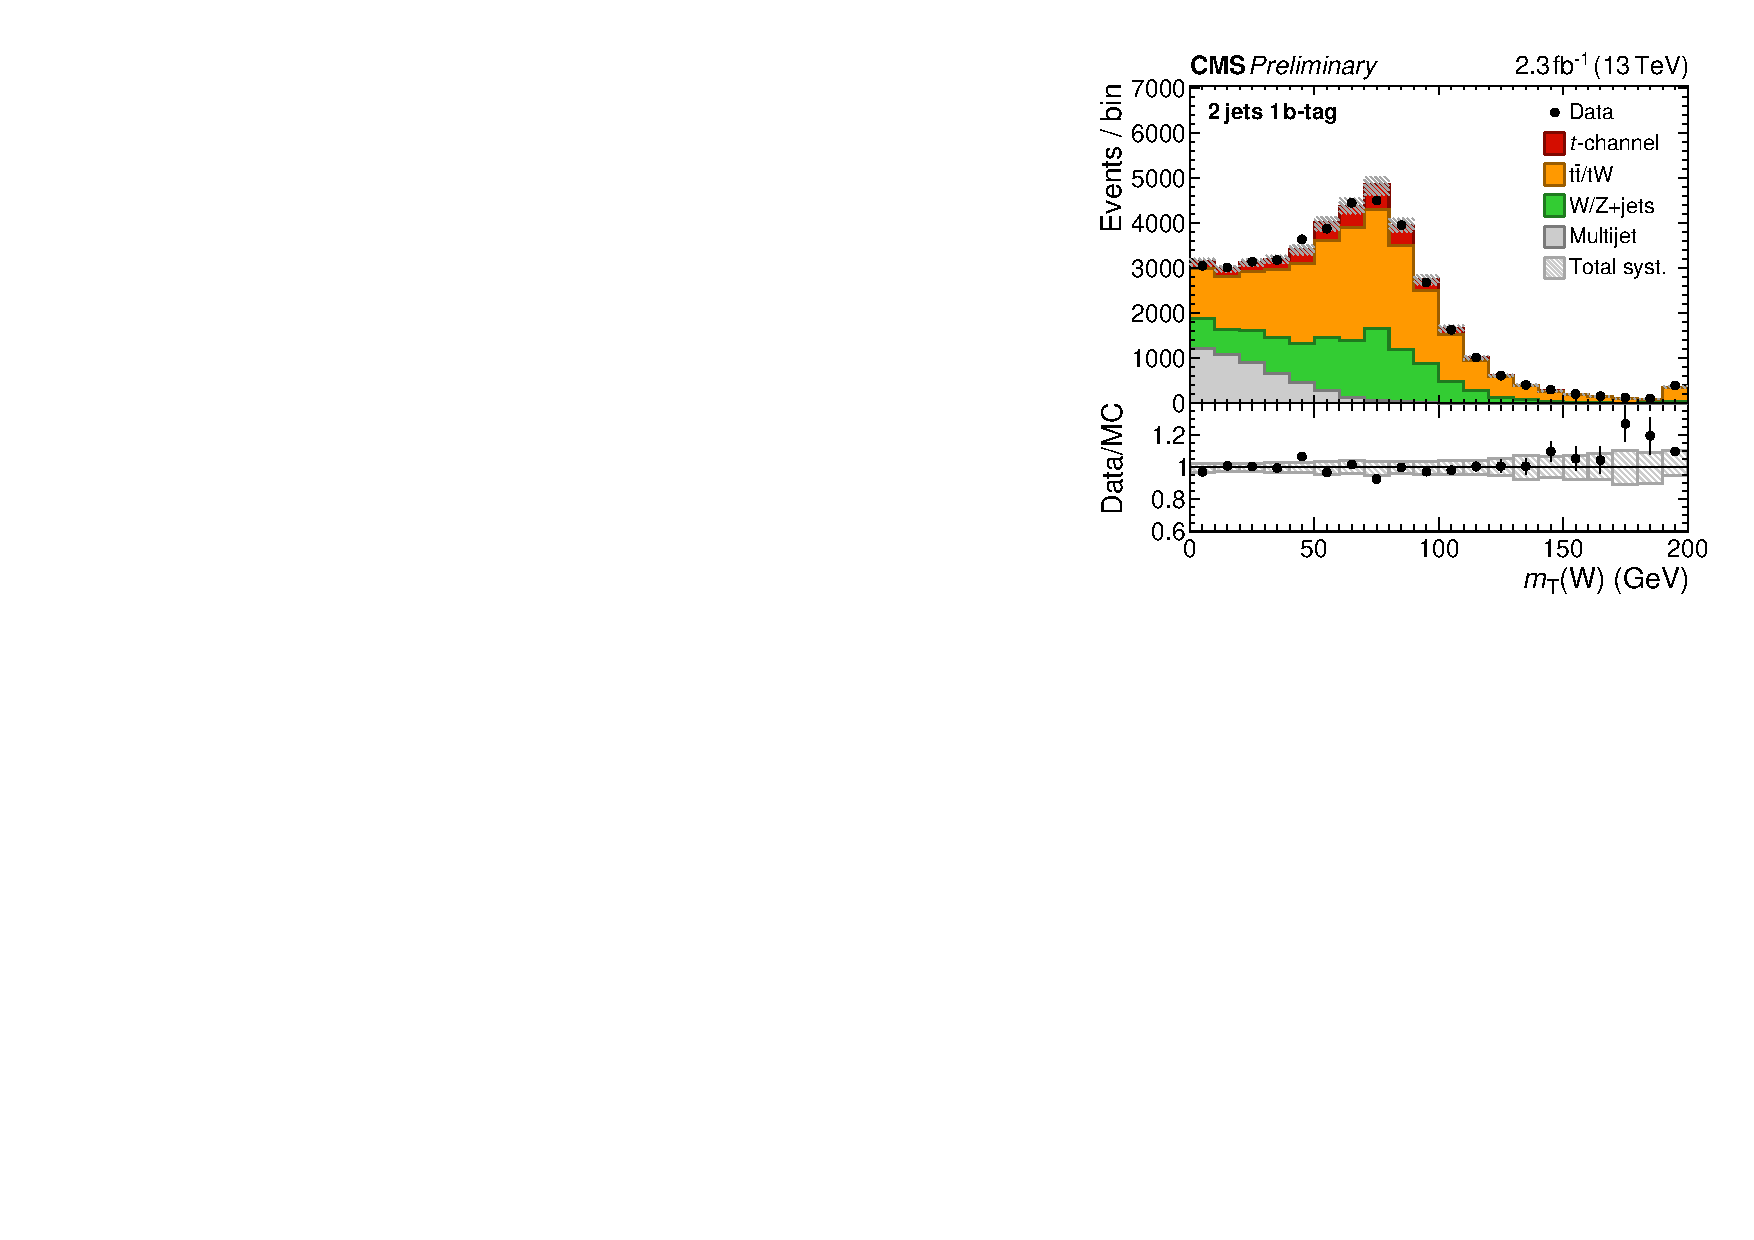
\includegraphics[width=0.48\textwidth]{figures/differential/pas/reco_mtw.pdf}}
\hspace{0.02\textwidth}
\subfloat[]{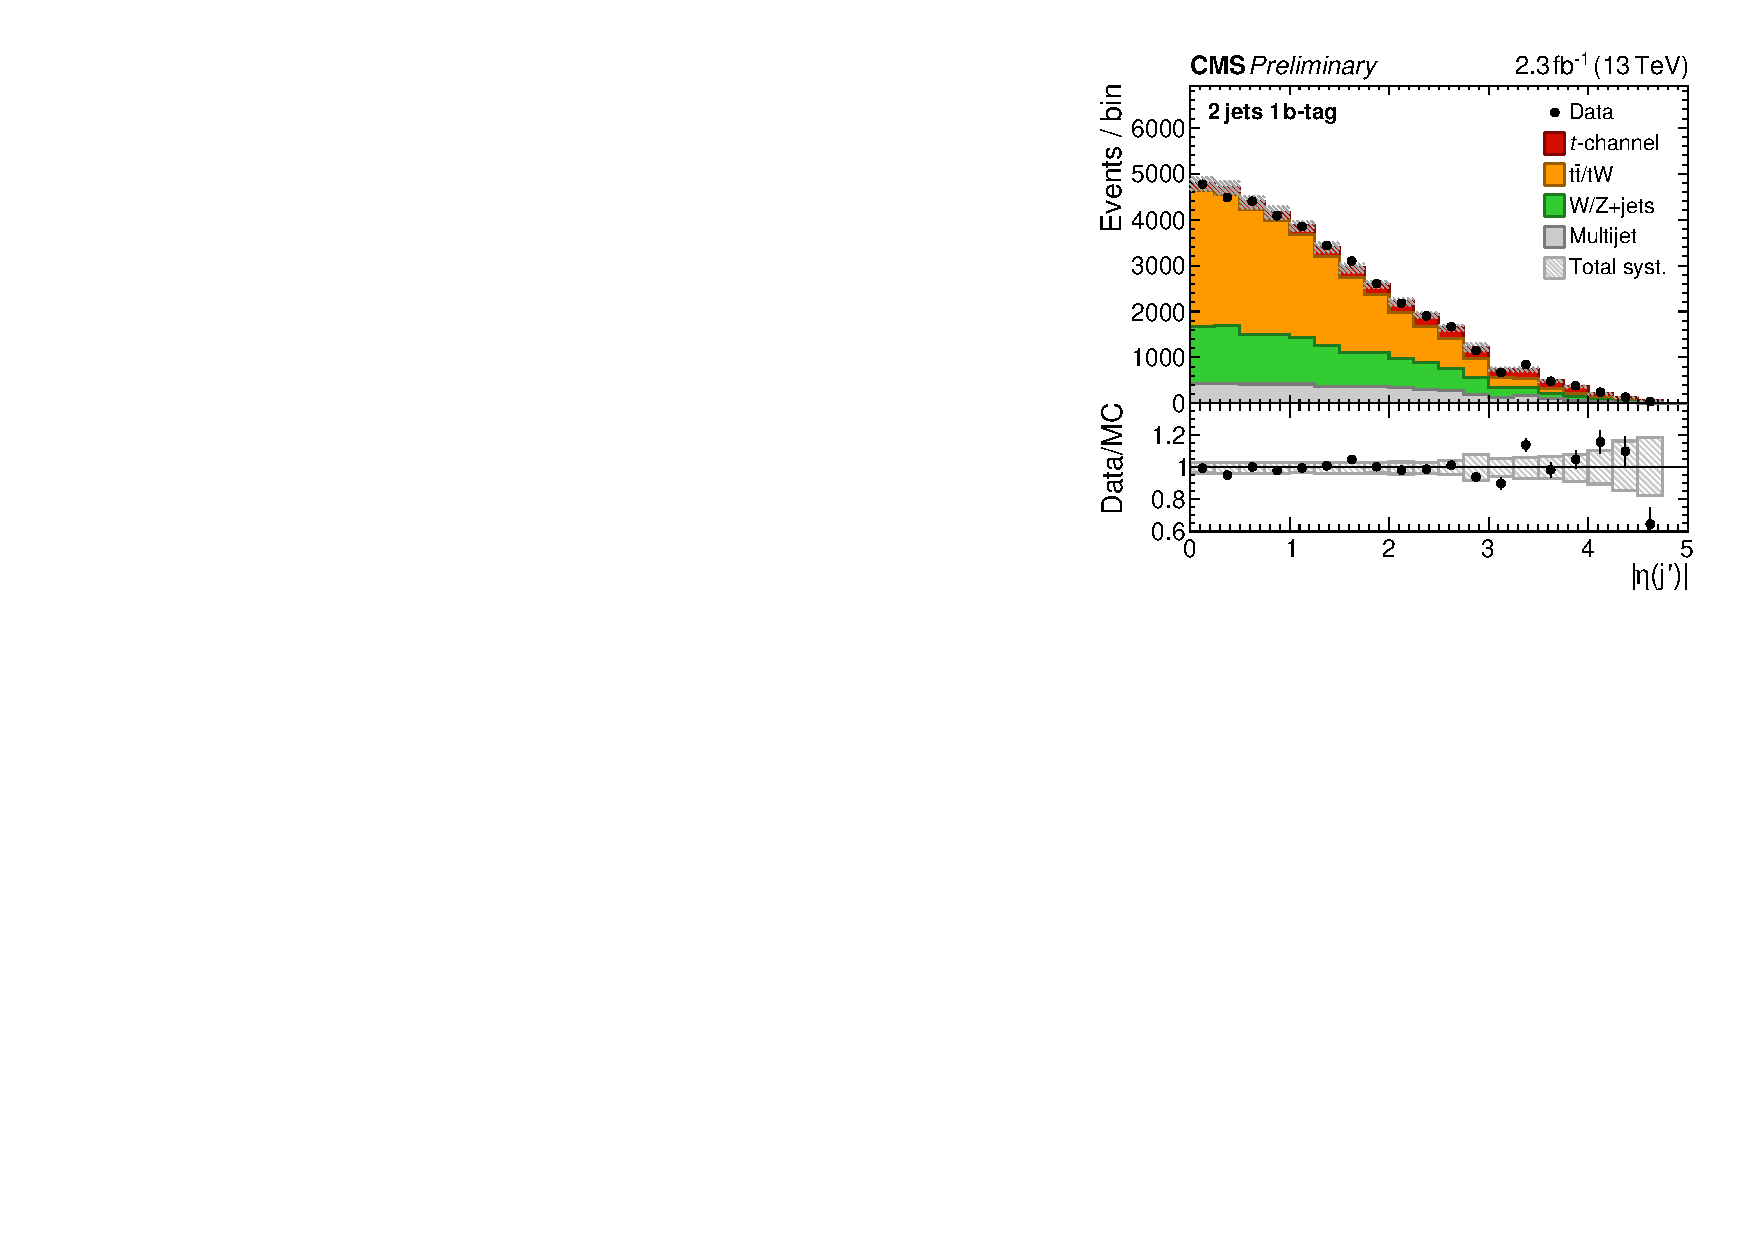
\includegraphics[width=0.48\textwidth]{figures/differential/pas/reco_etaj.pdf}}\\
\subfloat[]{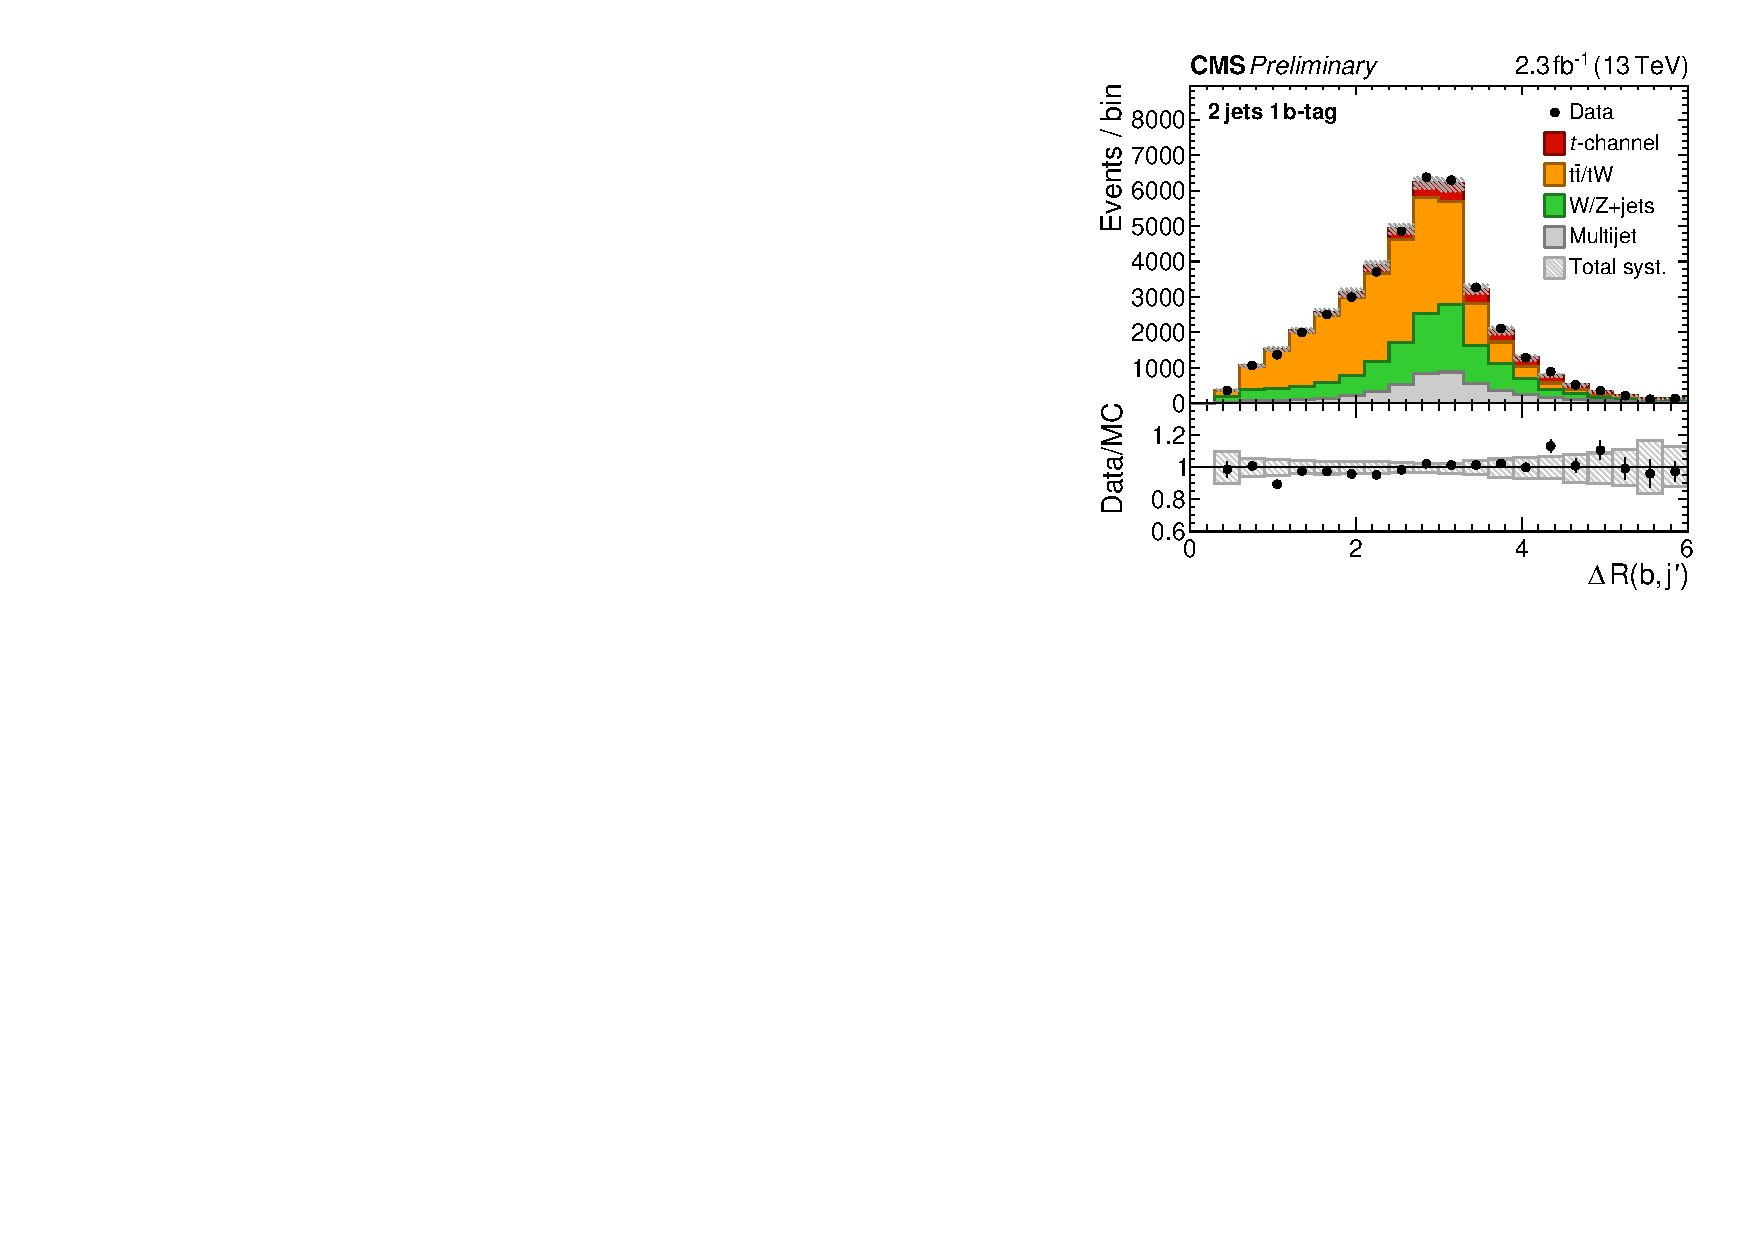
\includegraphics[width=0.48\textwidth]{figures/differential/pas/reco_dR.pdf}}
\hspace{0.02\textwidth}
\subfloat[]{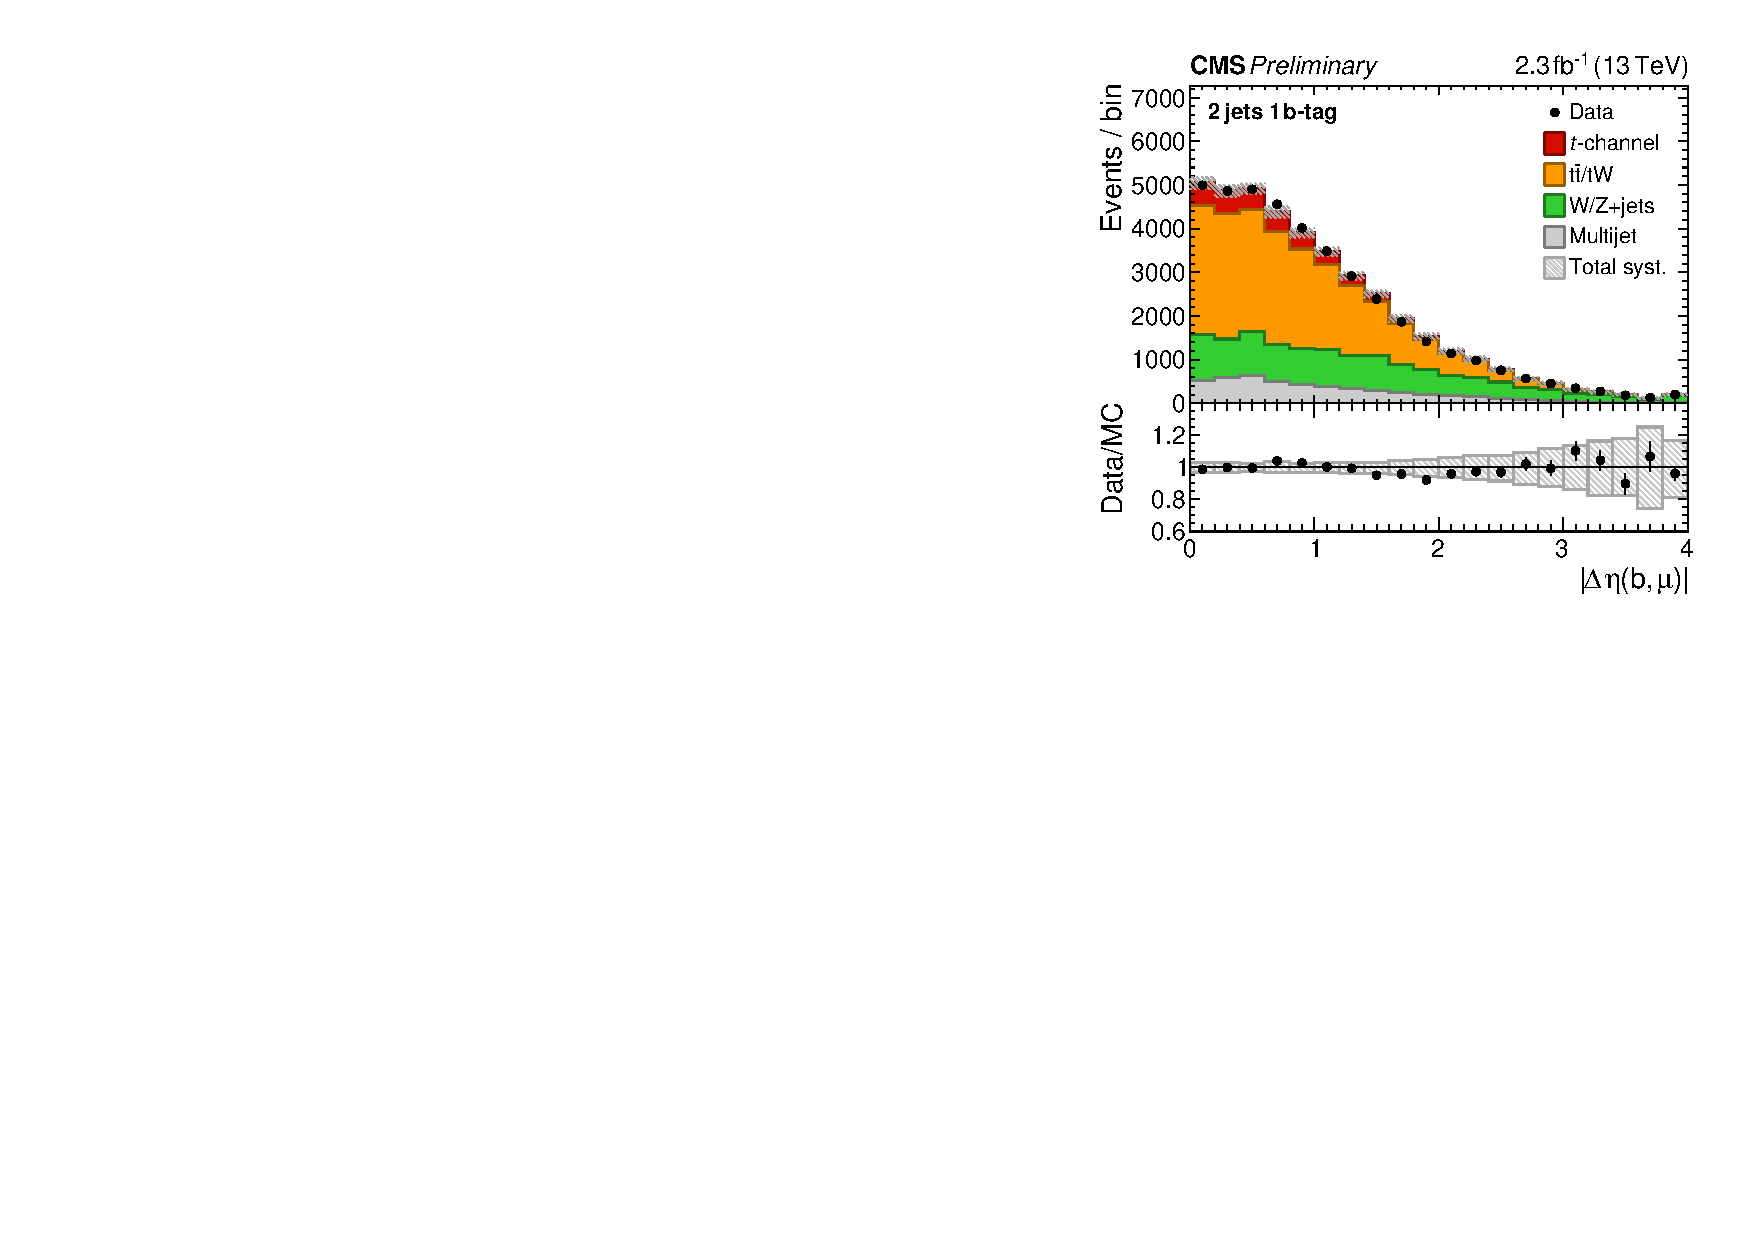
\includegraphics[width=0.48\textwidth]{figures/differential/pas/reco_dEta.pdf}}
}

\myfigure{\label{fig:diff13-bdt}Distribution of the \gls{bdt} discriminant after selecting events with $\mtw>50~\GeV$. The hatched band reflects the total systematic uncertainties. The figures are taken from Ref.~\cite{CMS-PAS-TOP-16-004}.}{
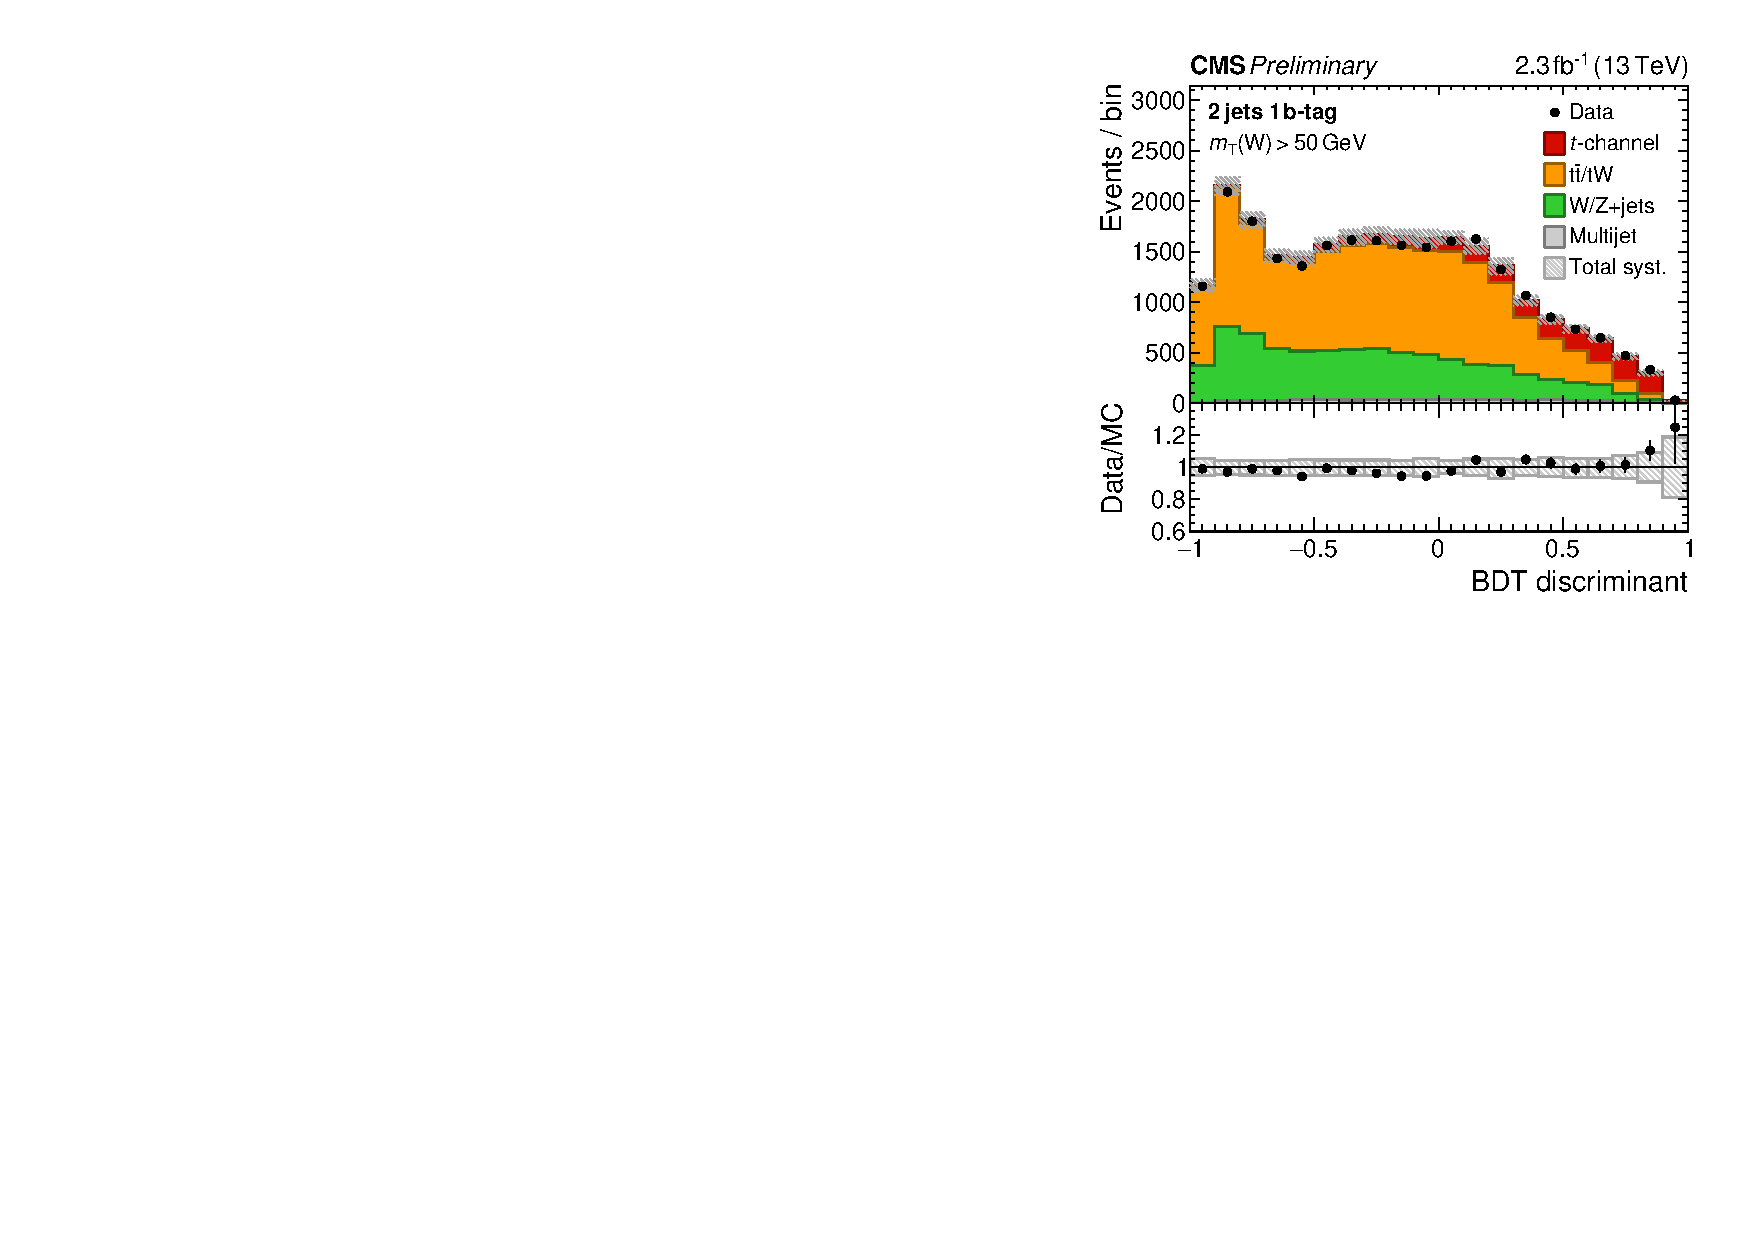
\includegraphics[width=0.48\textwidth]{figures/differential/pas/reco_BDT.pdf}
}

 bdt reshaping by multiplying factors and tanh, correlation with top pt and y

%##############################################
\section{Signal extraction}
%##############################################
\label{sec:diff13-fit}

\mytable{Estimated event yields in 2j1t after the event selection, for events with $\mtw>50~\GeV$, and in a signal-enriched phase space defined by $\mtw>50~\GeV$ and $\bdt>0.6$\,.}{
\begin{tabular}{@{}l l r@{$\pm$}l c r@{$\pm$}l c r@{$\pm$}l@{}}
\toprule
Process &\hspace*{0.3cm}&\multicolumn{8}{c@{}}{Event yields}  \\
\cmidrule{3-10}
&&\multicolumn{2}{c}{Selection} &\hspace*{0.2cm}& \multicolumn{2}{c}{$\mtw>50~\GeV$} &\hspace*{0.2cm}& \multicolumn{2}{c@{}}{Signal-enriched}\\
\midrule
tW              &&\hspace*{0.1cm} 2001&14      &&\hspace*{0.5cm} 1343&12       &&\hspace*{0.6cm} 32&2\\
\ttbar          && 19037&22     && 12960&18      && 353&3\\
W+heavy flavor  && 6825&57      && 4807&49       && 189&11 \\
W+light flavor  && 2395&40      && 1684&34       && 71&7 \\
\zjets          && 1534&24      && 664&16        && 23&3 \\
Multijet        && 4881&18      && 561&3         && 38&1\\
Signal          && 3385&5       && 2351&4        && 700&2\\
\midrule
Total expected  && 40057&80     && 24369&66      && 1407&13\\
Data            && 40432&201    && 24417&156     && 1482&38 \\
\bottomrule
\end{tabular}
}

\myfigure{Correlations between fitted scale factors.}{
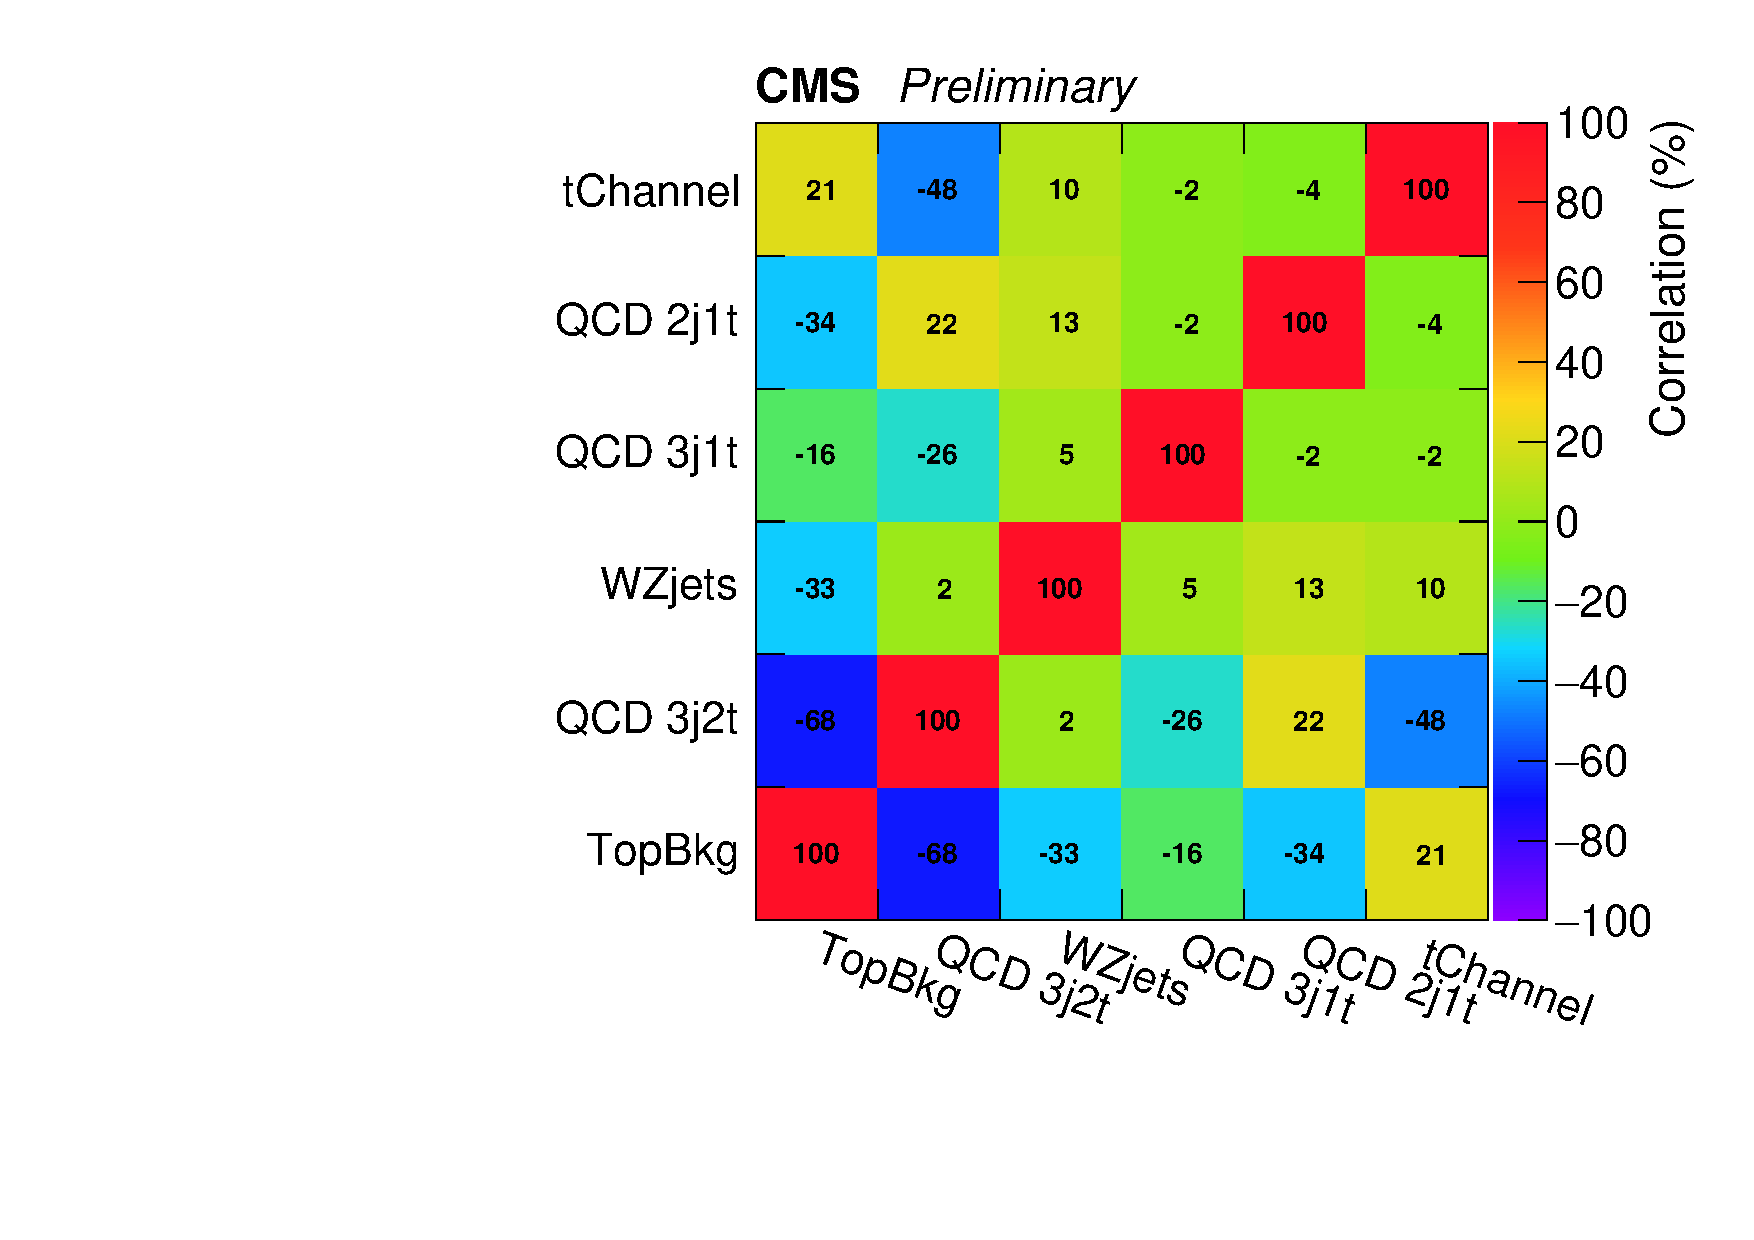
\includegraphics[width=0.5\textwidth]{figures/differential/fitCorrelations.pdf}
}



%##############################################
\section{Unfolding}
%##############################################

\myfigure{Response matrices for the top-quark (a)~transverse momentum and (b)~rapidity.}{
\subfloat[]{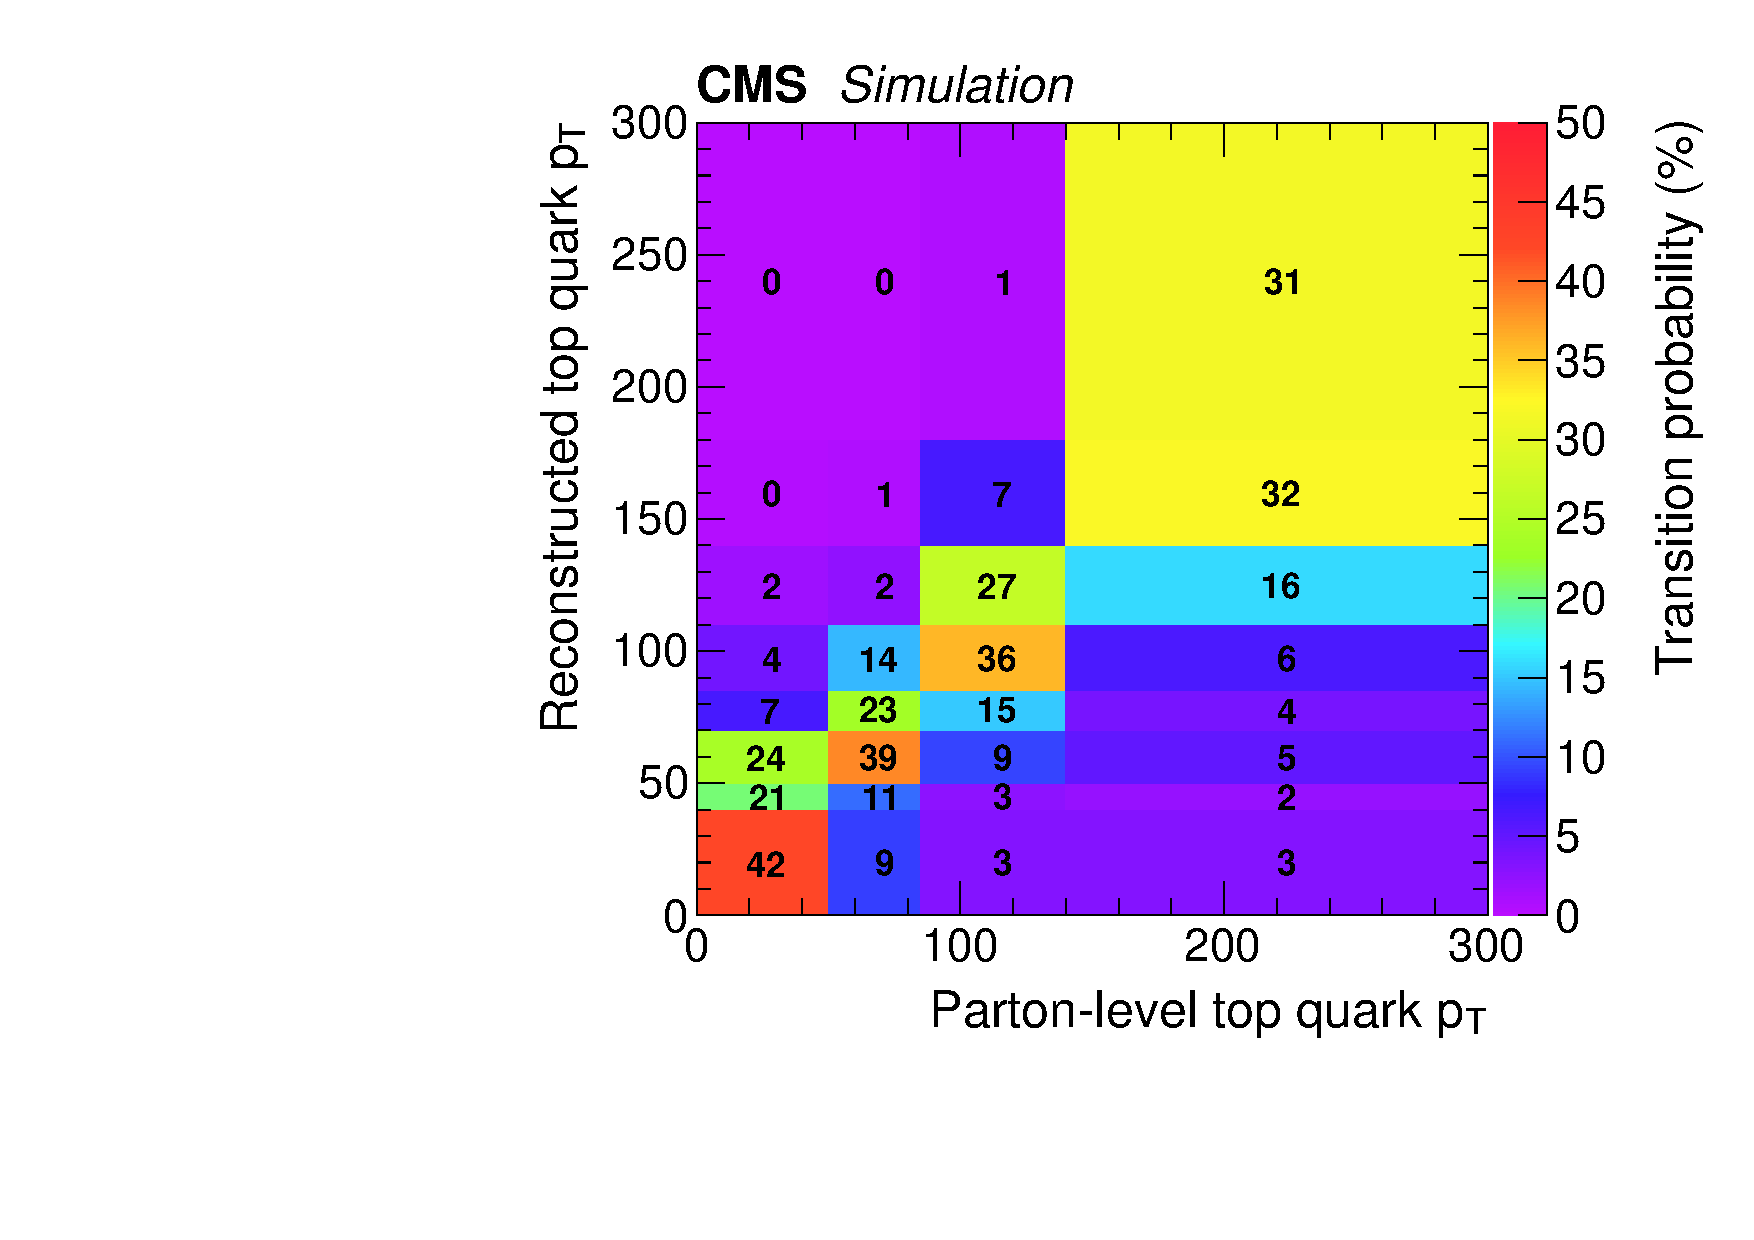
\includegraphics[width=0.48\textwidth]{figures/differential/unfolding/responsePt.pdf}}
\hspace{0.02\textwidth}
\subfloat[]{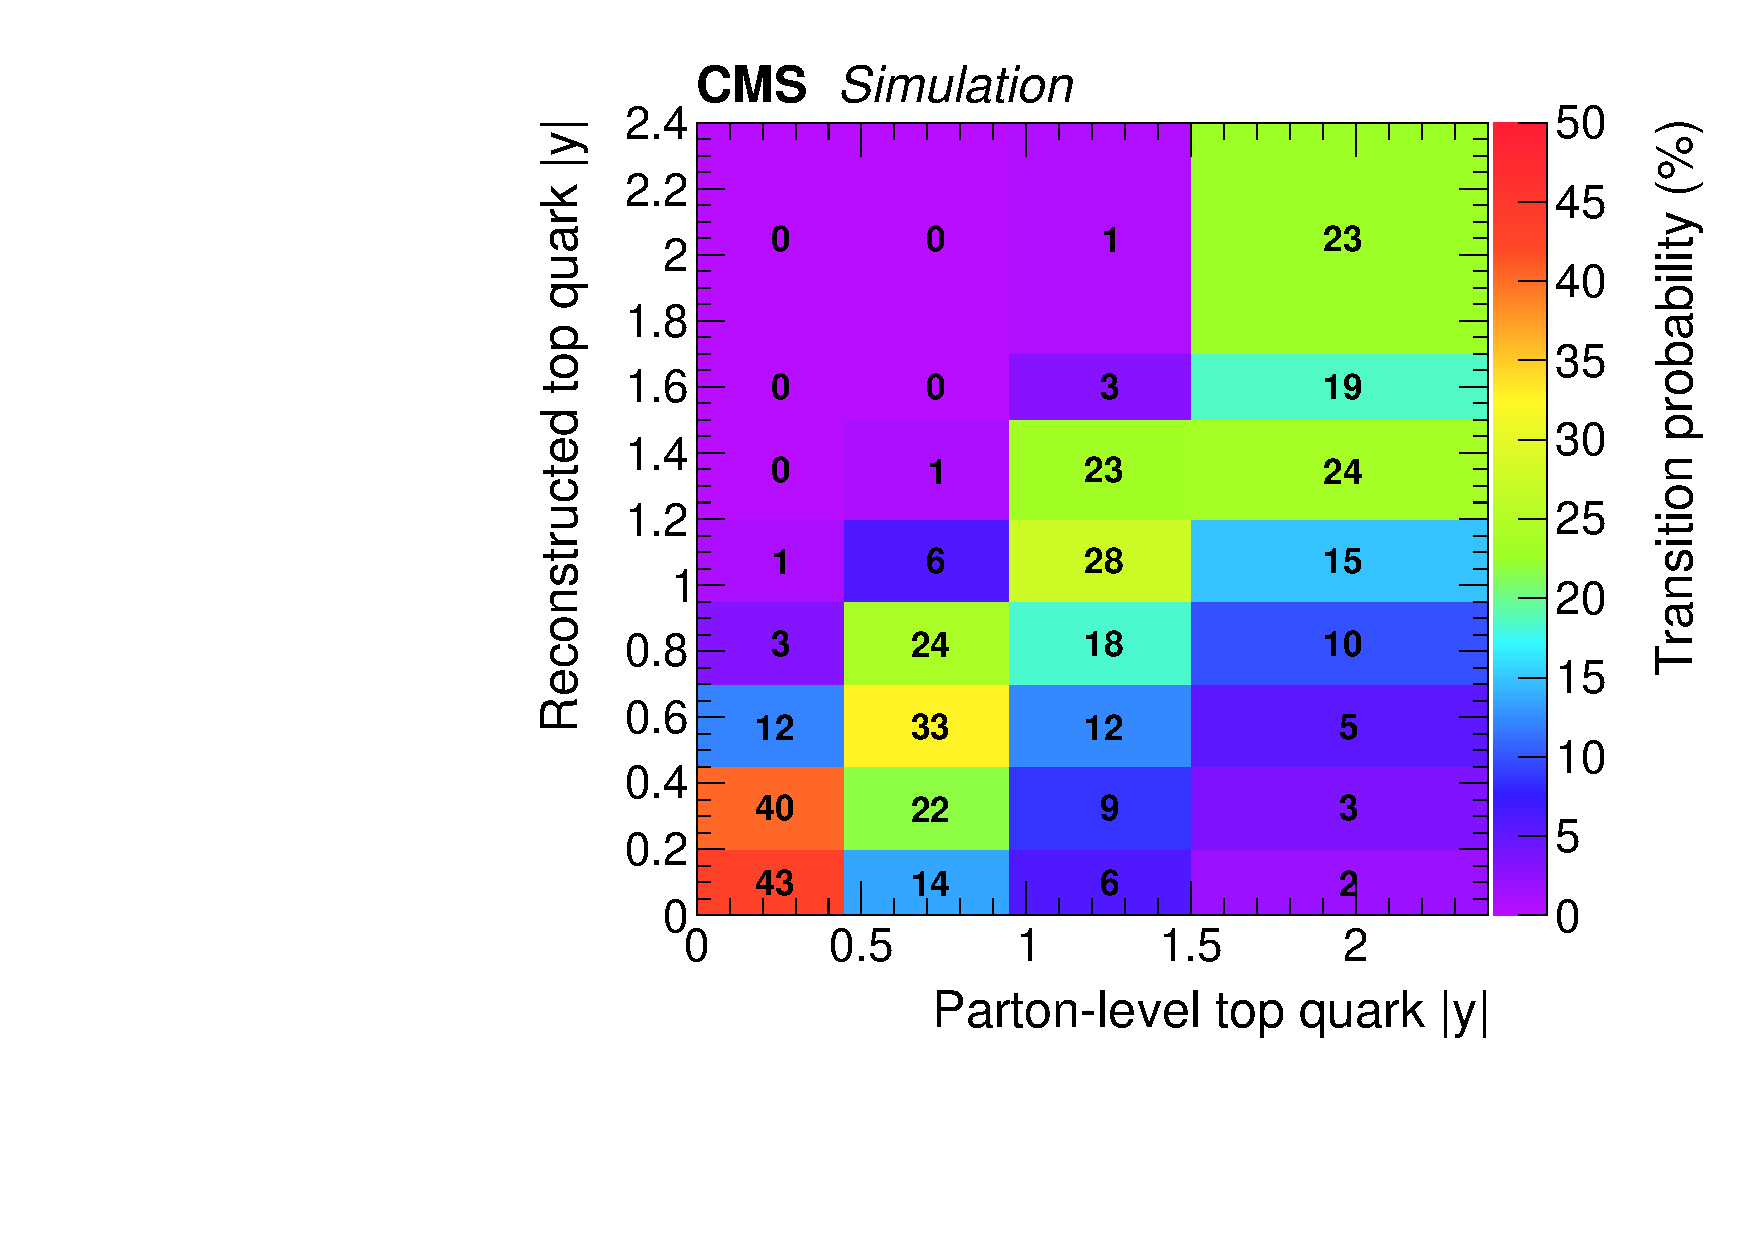
\includegraphics[width=0.48\textwidth]{figures/differential/unfolding/responseY.pdf}}
}

\myfigure{Selection efficiencies for the top-quark (a)~transverse momentum and (b)~rapidity.}{
\subfloat[]{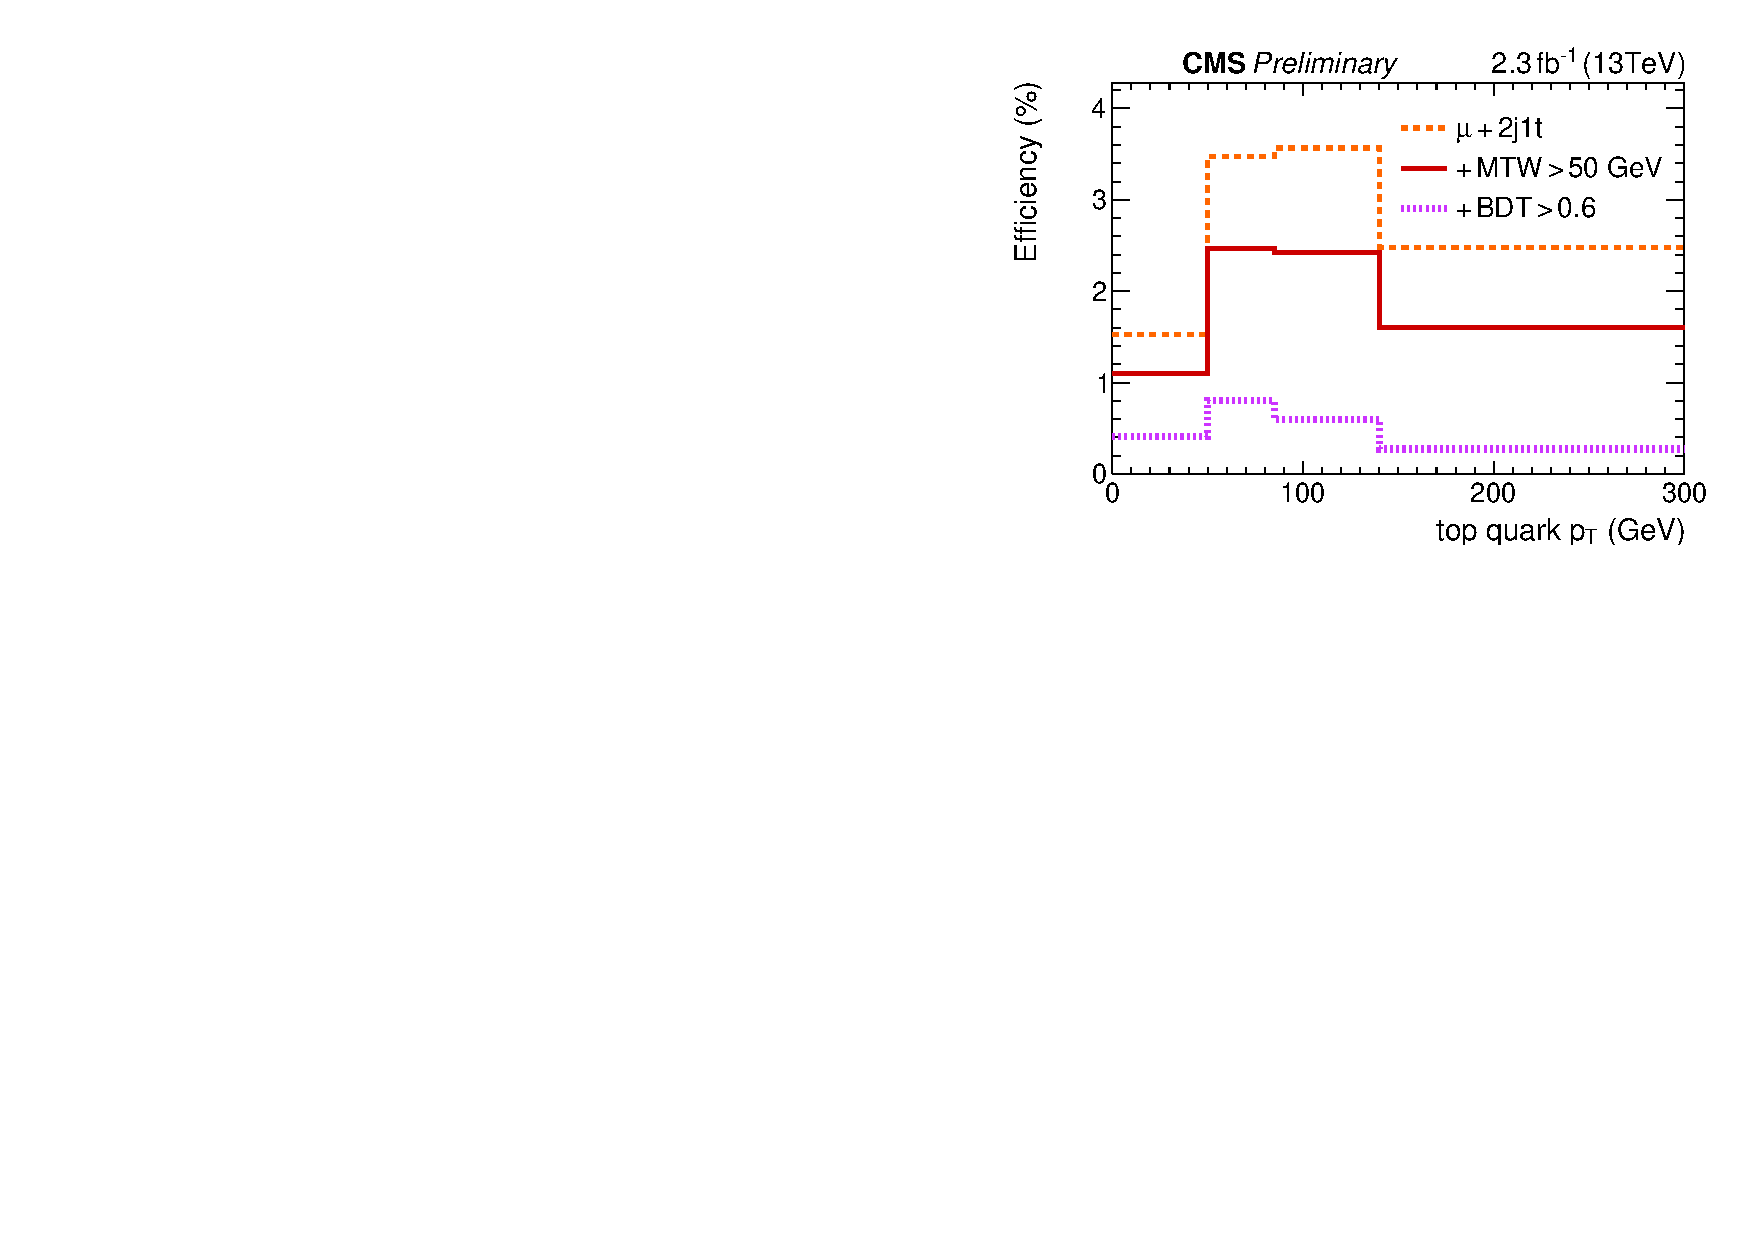
\includegraphics[width=0.48\textwidth]{figures/differential/unfolding/effPt.pdf}}
\hspace{0.02\textwidth}
\subfloat[]{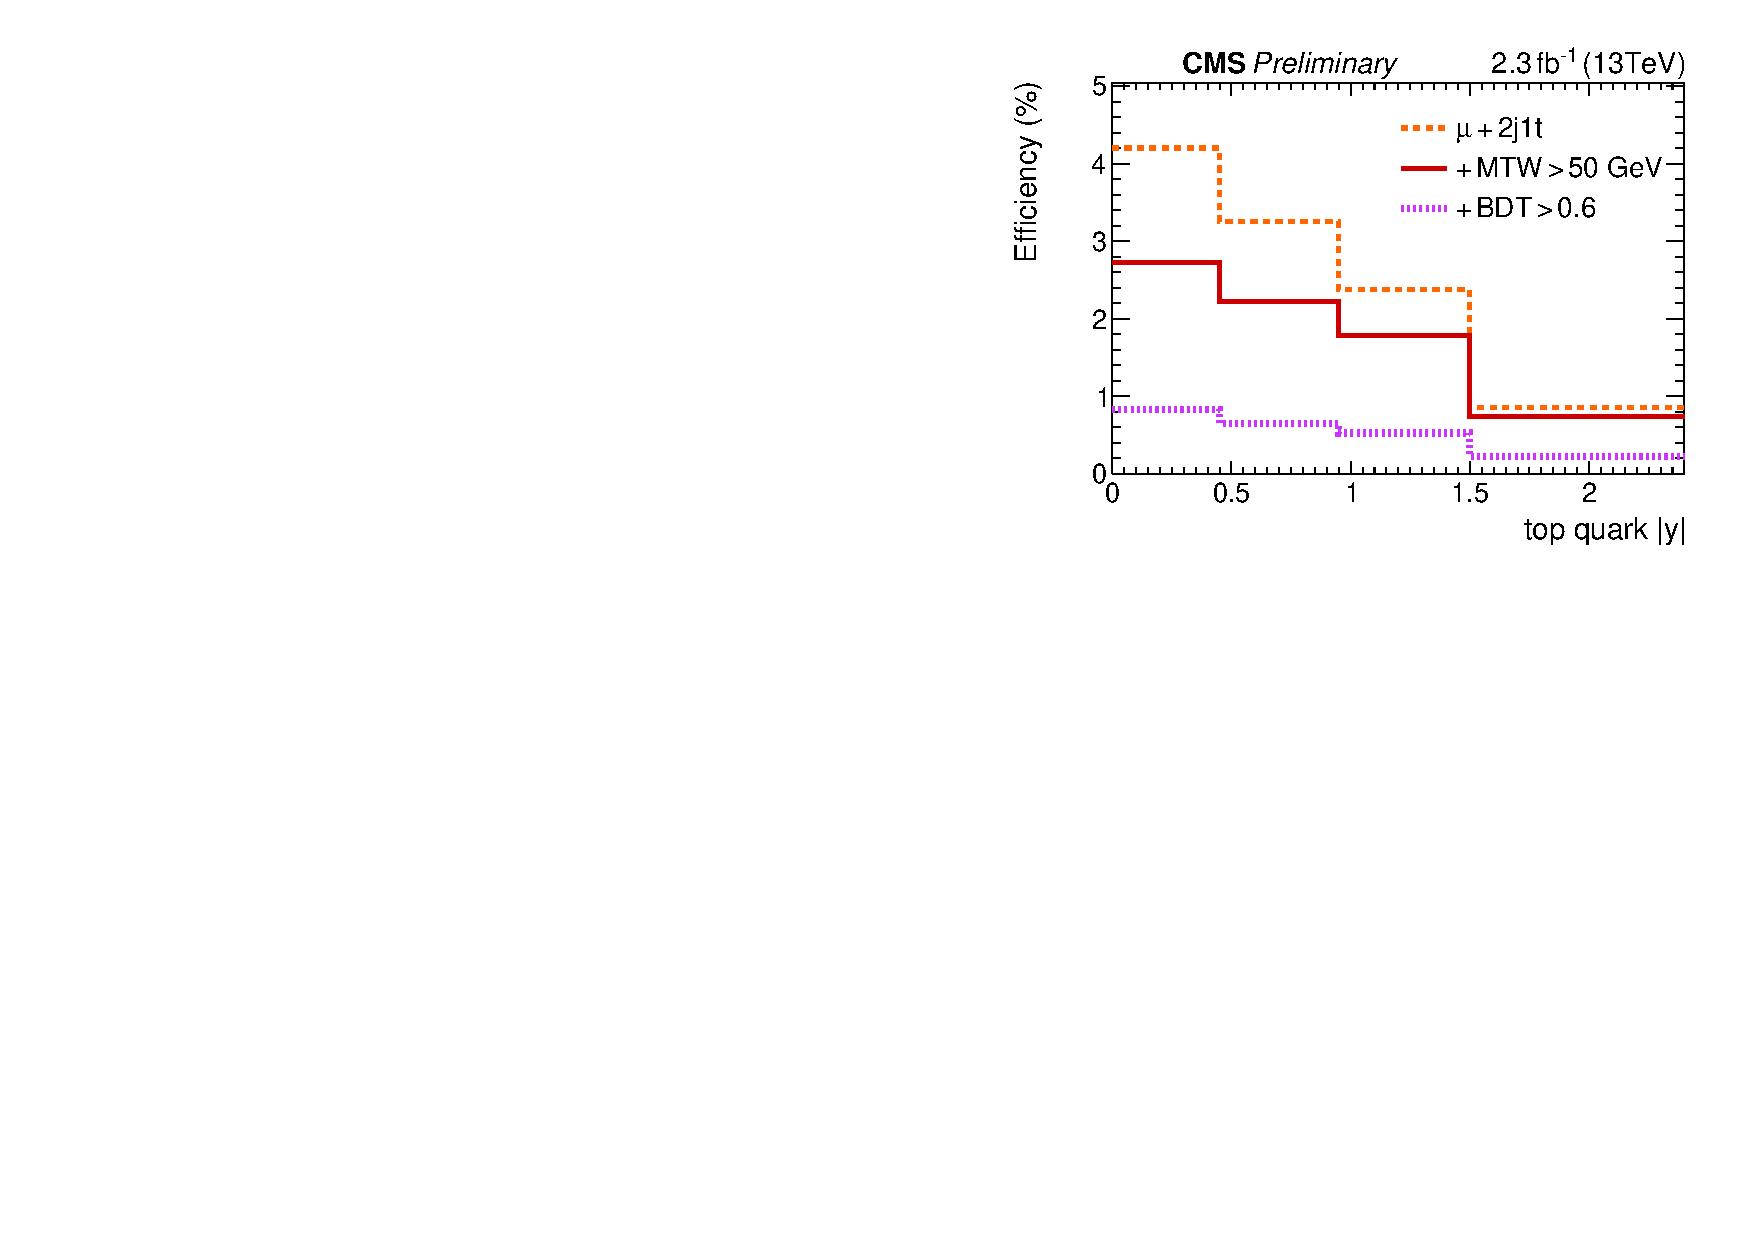
\includegraphics[width=0.48\textwidth]{figures/differential/unfolding/effY.pdf}}
}

\myfigure{\label{fig:diff13-top-reco} ??? The hatched band reflects the total systematic uncertainties. The figures are taken from Ref.~\cite{CMS-PAS-TOP-16-004}.}{
\subfloat[]{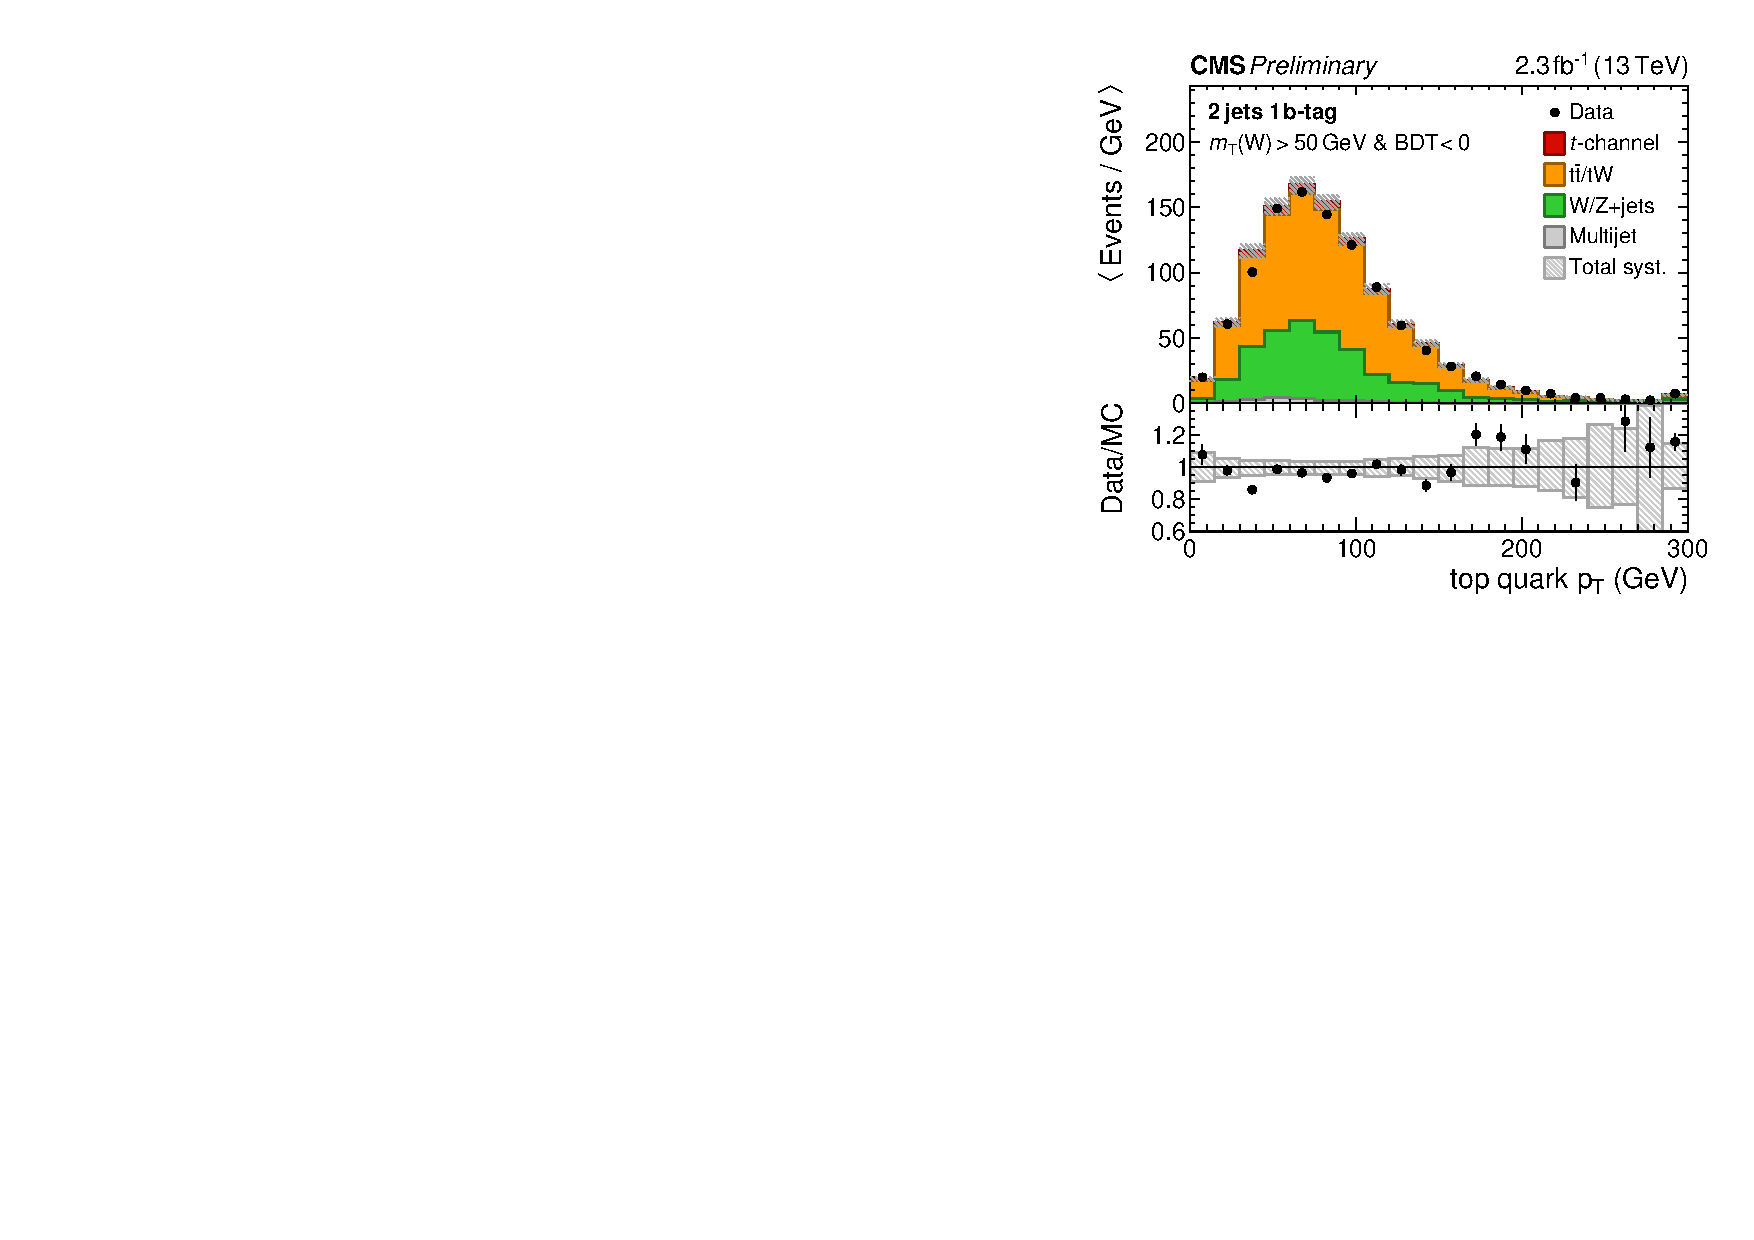
\includegraphics[width=0.48\textwidth]{figures/differential/pas/reco_toppt_bdtinv.pdf}}
\hspace{0.02\textwidth}
\subfloat[]{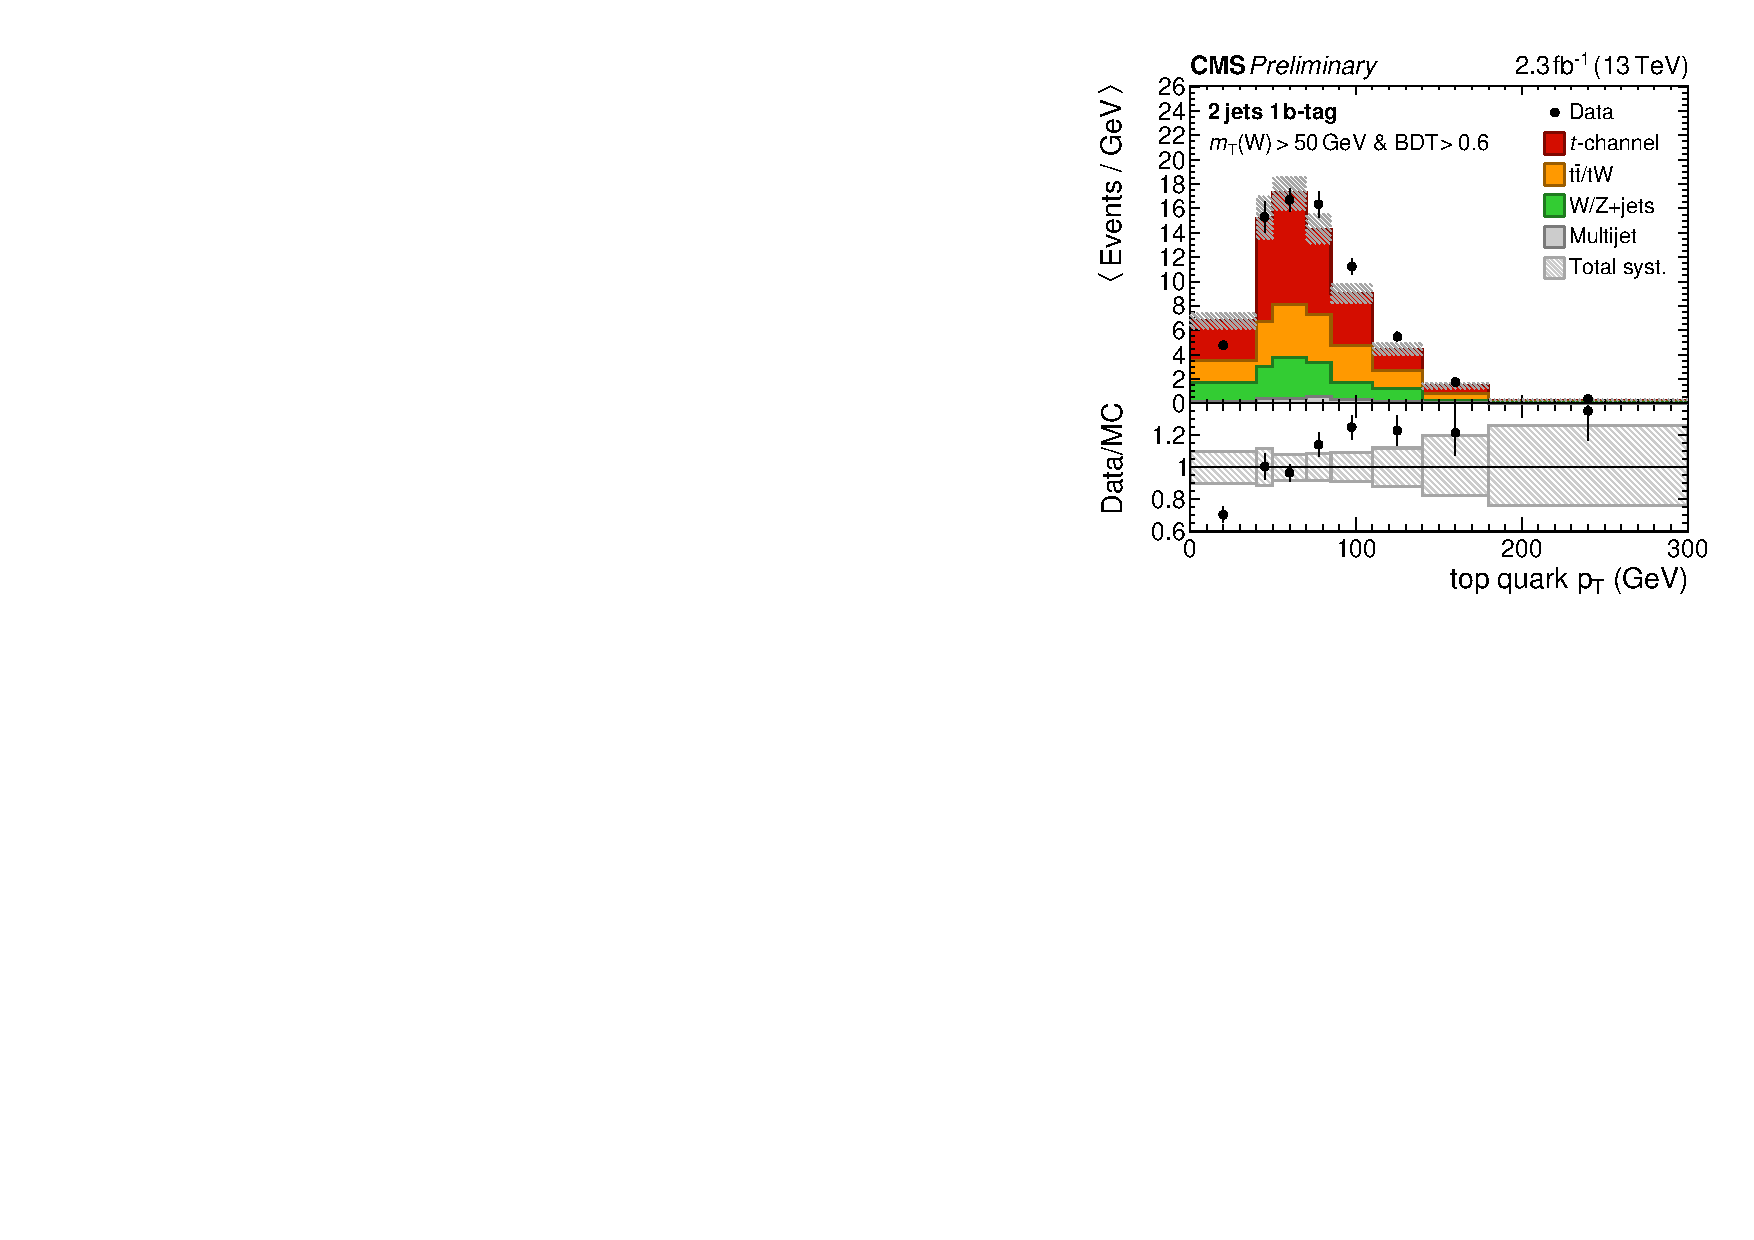
\includegraphics[width=0.48\textwidth]{figures/differential/pas/reco_toppt_bdt.pdf}}\\
\subfloat[]{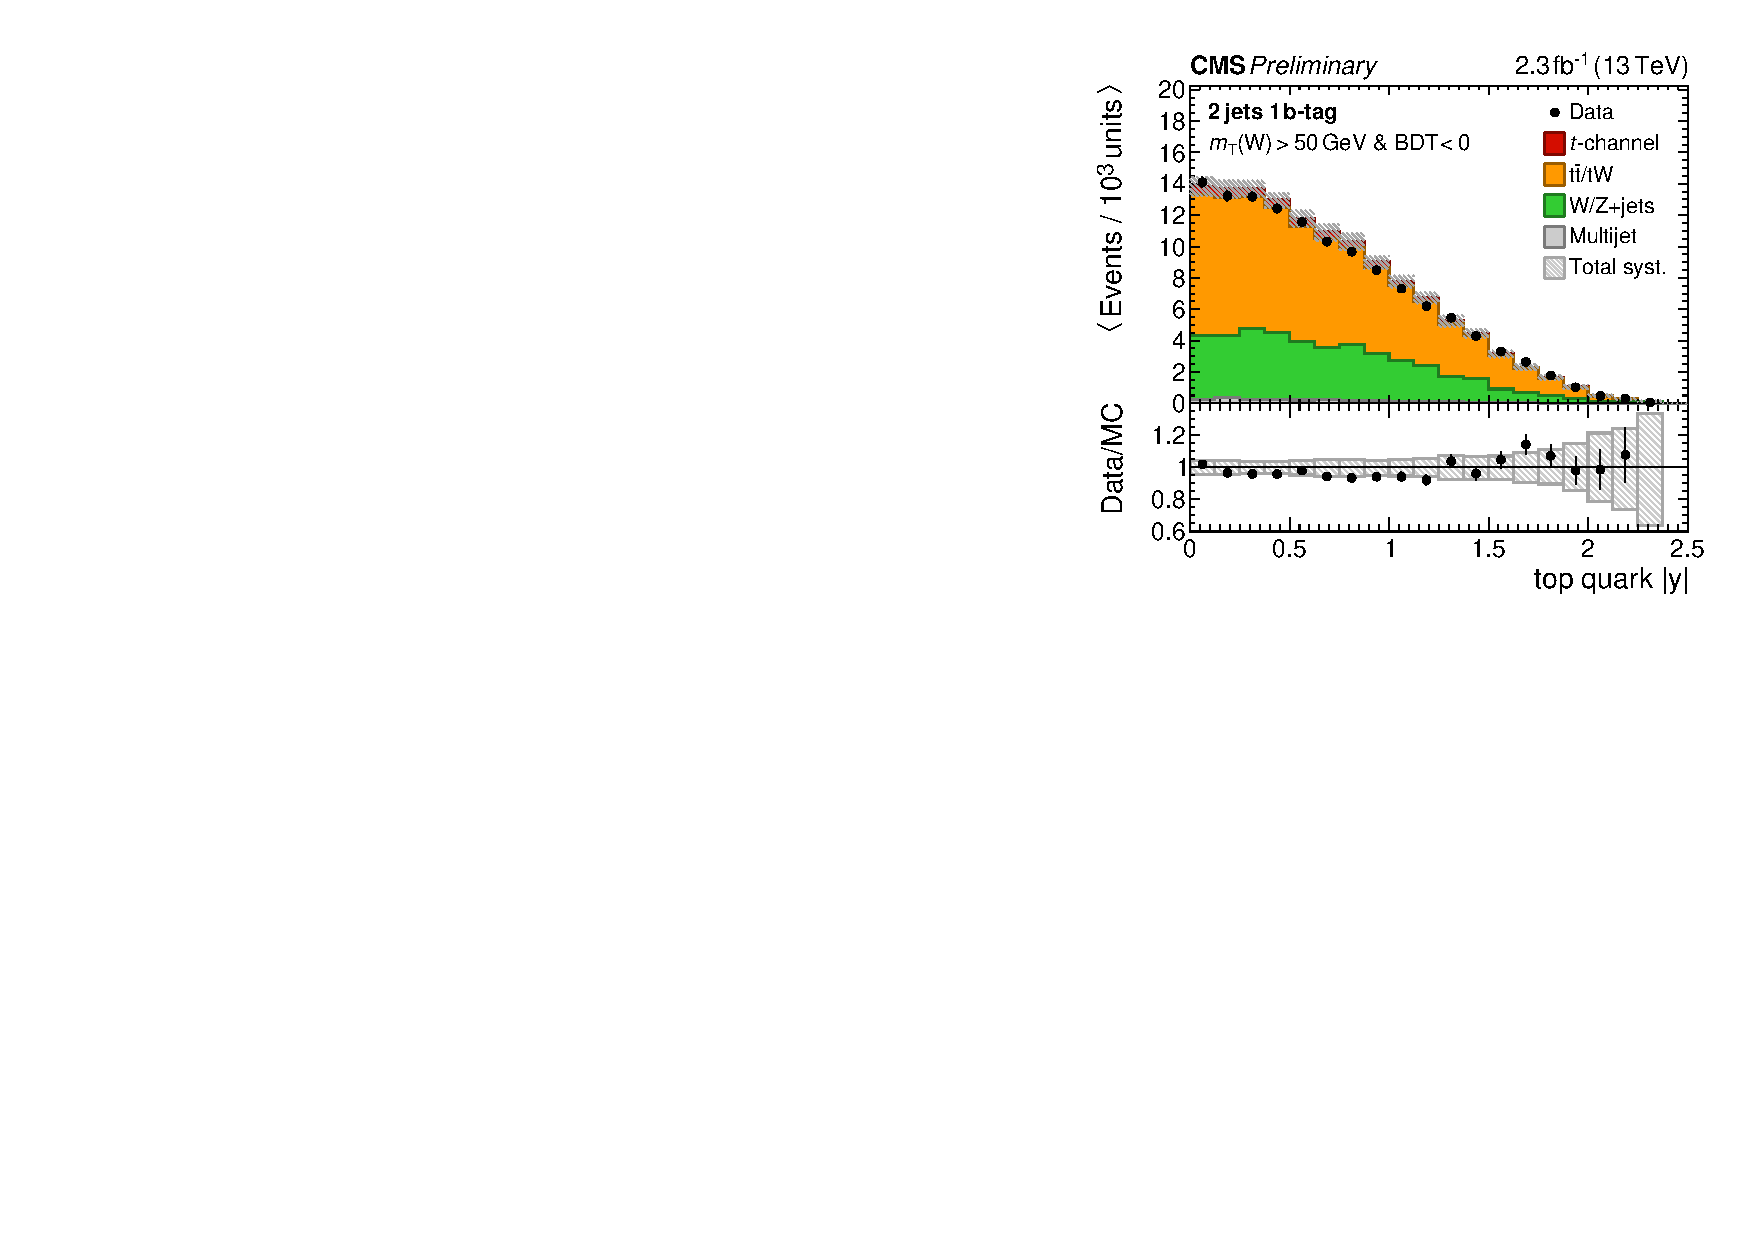
\includegraphics[width=0.48\textwidth]{figures/differential/pas/reco_topy_bdtinv.pdf}}
\hspace{0.02\textwidth}
\subfloat[]{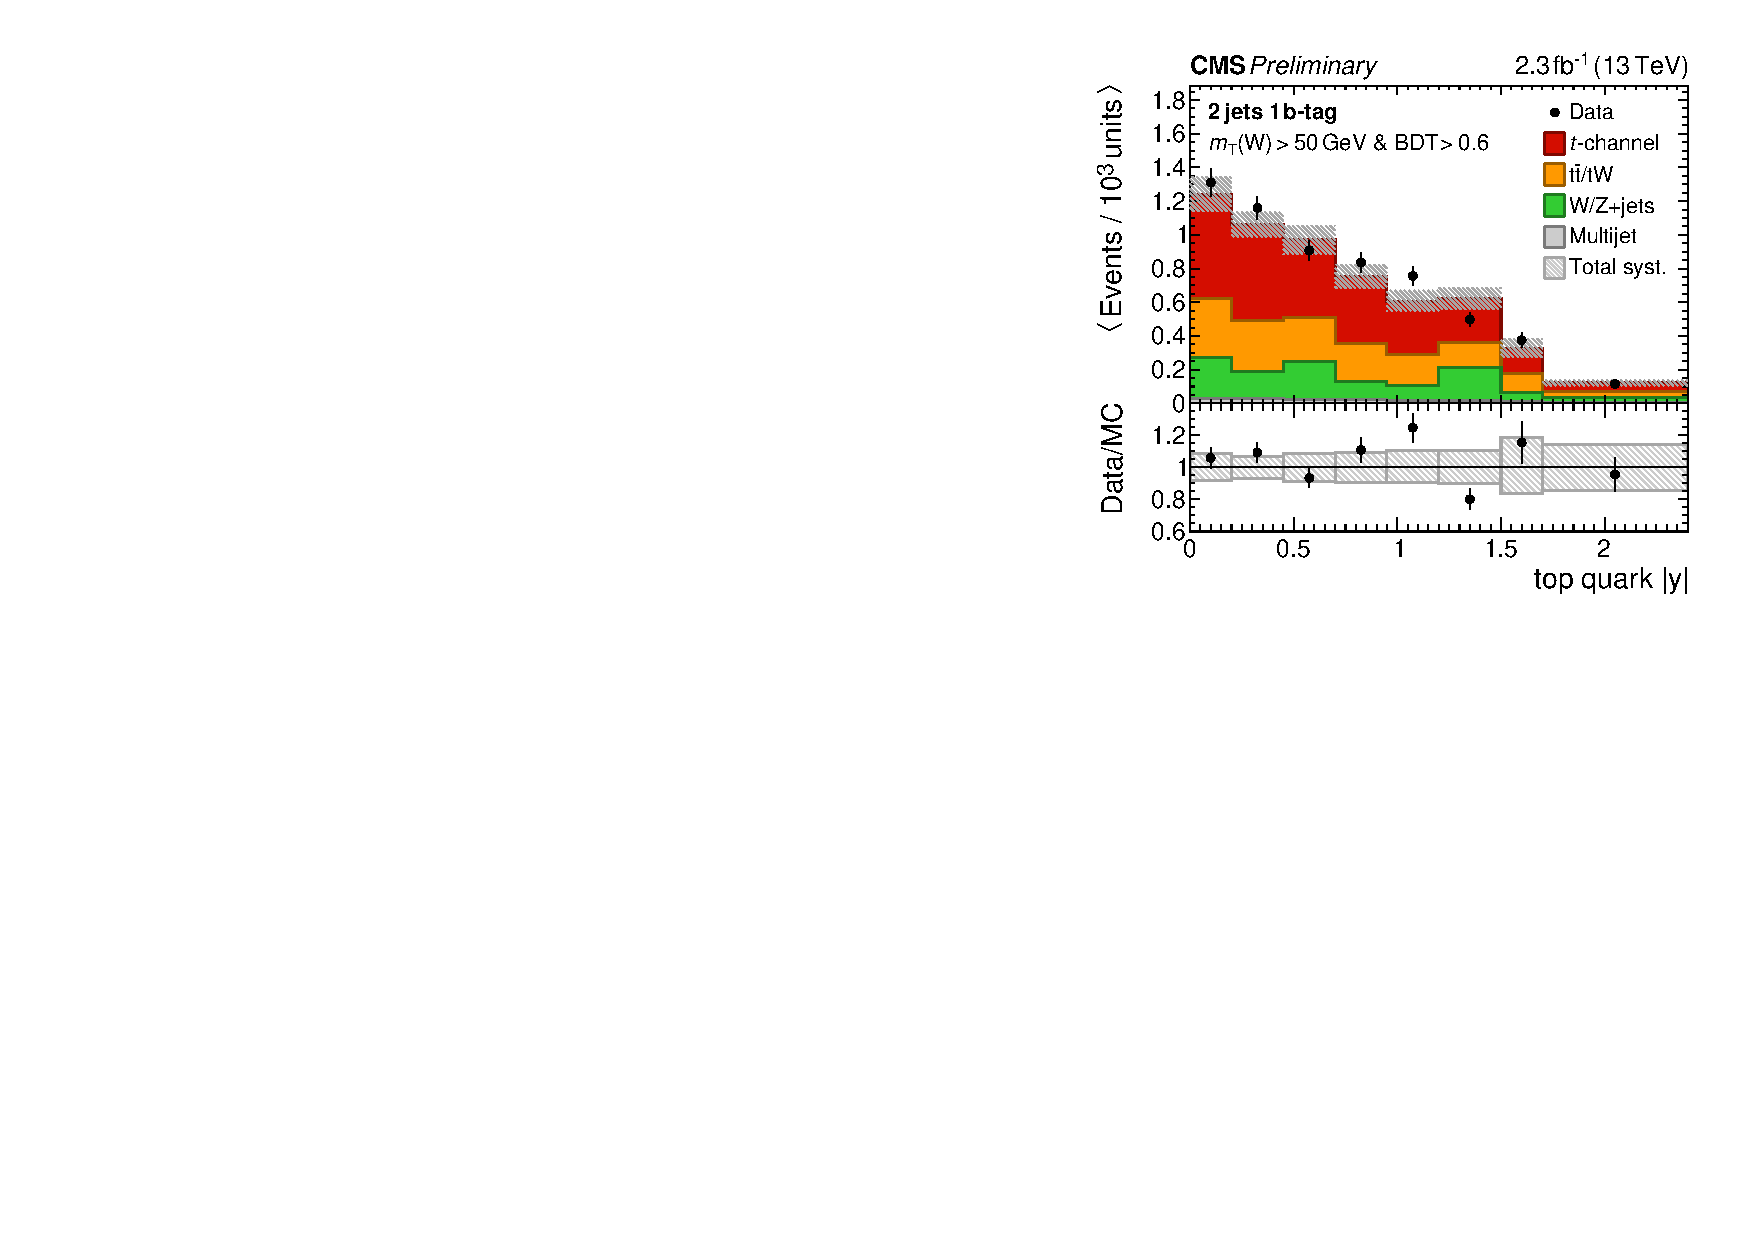
\includegraphics[width=0.48\textwidth]{figures/differential/pas/reco_topy_bdt.pdf}}
}

\myfigure{\label{fig:diff13-top-reco-3j1t} .}{
\subfloat[]{\adjincludegraphics[height=4.8cm,trim={0 0 {0.16\width} 0},clip]{figures/differential/plots/3j1t/3j1t_top_pt_qcdnone_nol.pdf}}
\subfloat[]{\adjincludegraphics[height=4.8cm,trim={0 0 {0.\width} 0},clip]{figures/differential/plots/3j1t/3j1t_top_absy_qcdnone.pdf}}
}


pulls, binning choice, how is rapidity defined, tau scan

%##############################################
\section{Statistical evaluation}
%##############################################

show impact of uncertainties on shape

\myfigure{\label{fig:diff13-top-pt-sys} .}{
\subfloat[]{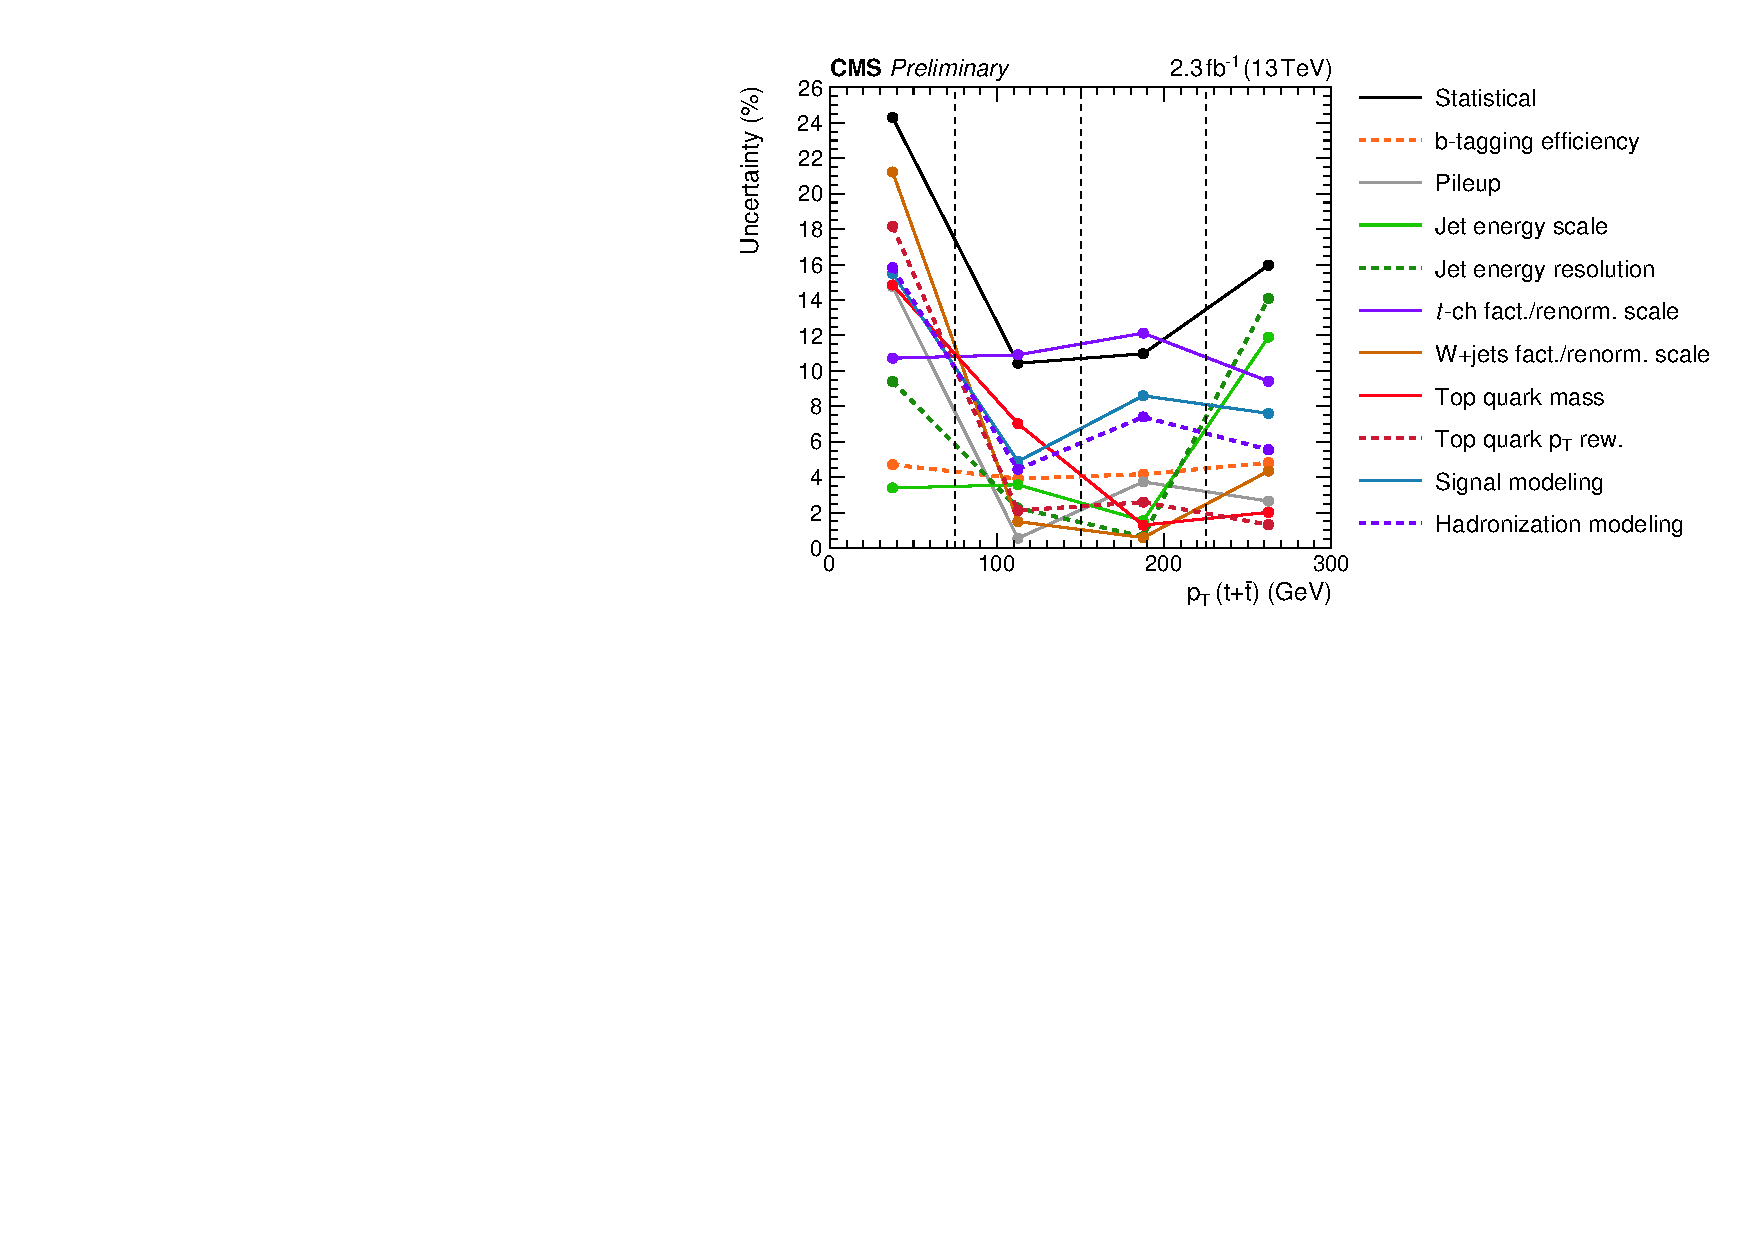
\includegraphics[width=0.9\textwidth]{figures/differential/unfolding/unfolded_top_pt_unc.pdf}}\\
\subfloat[]{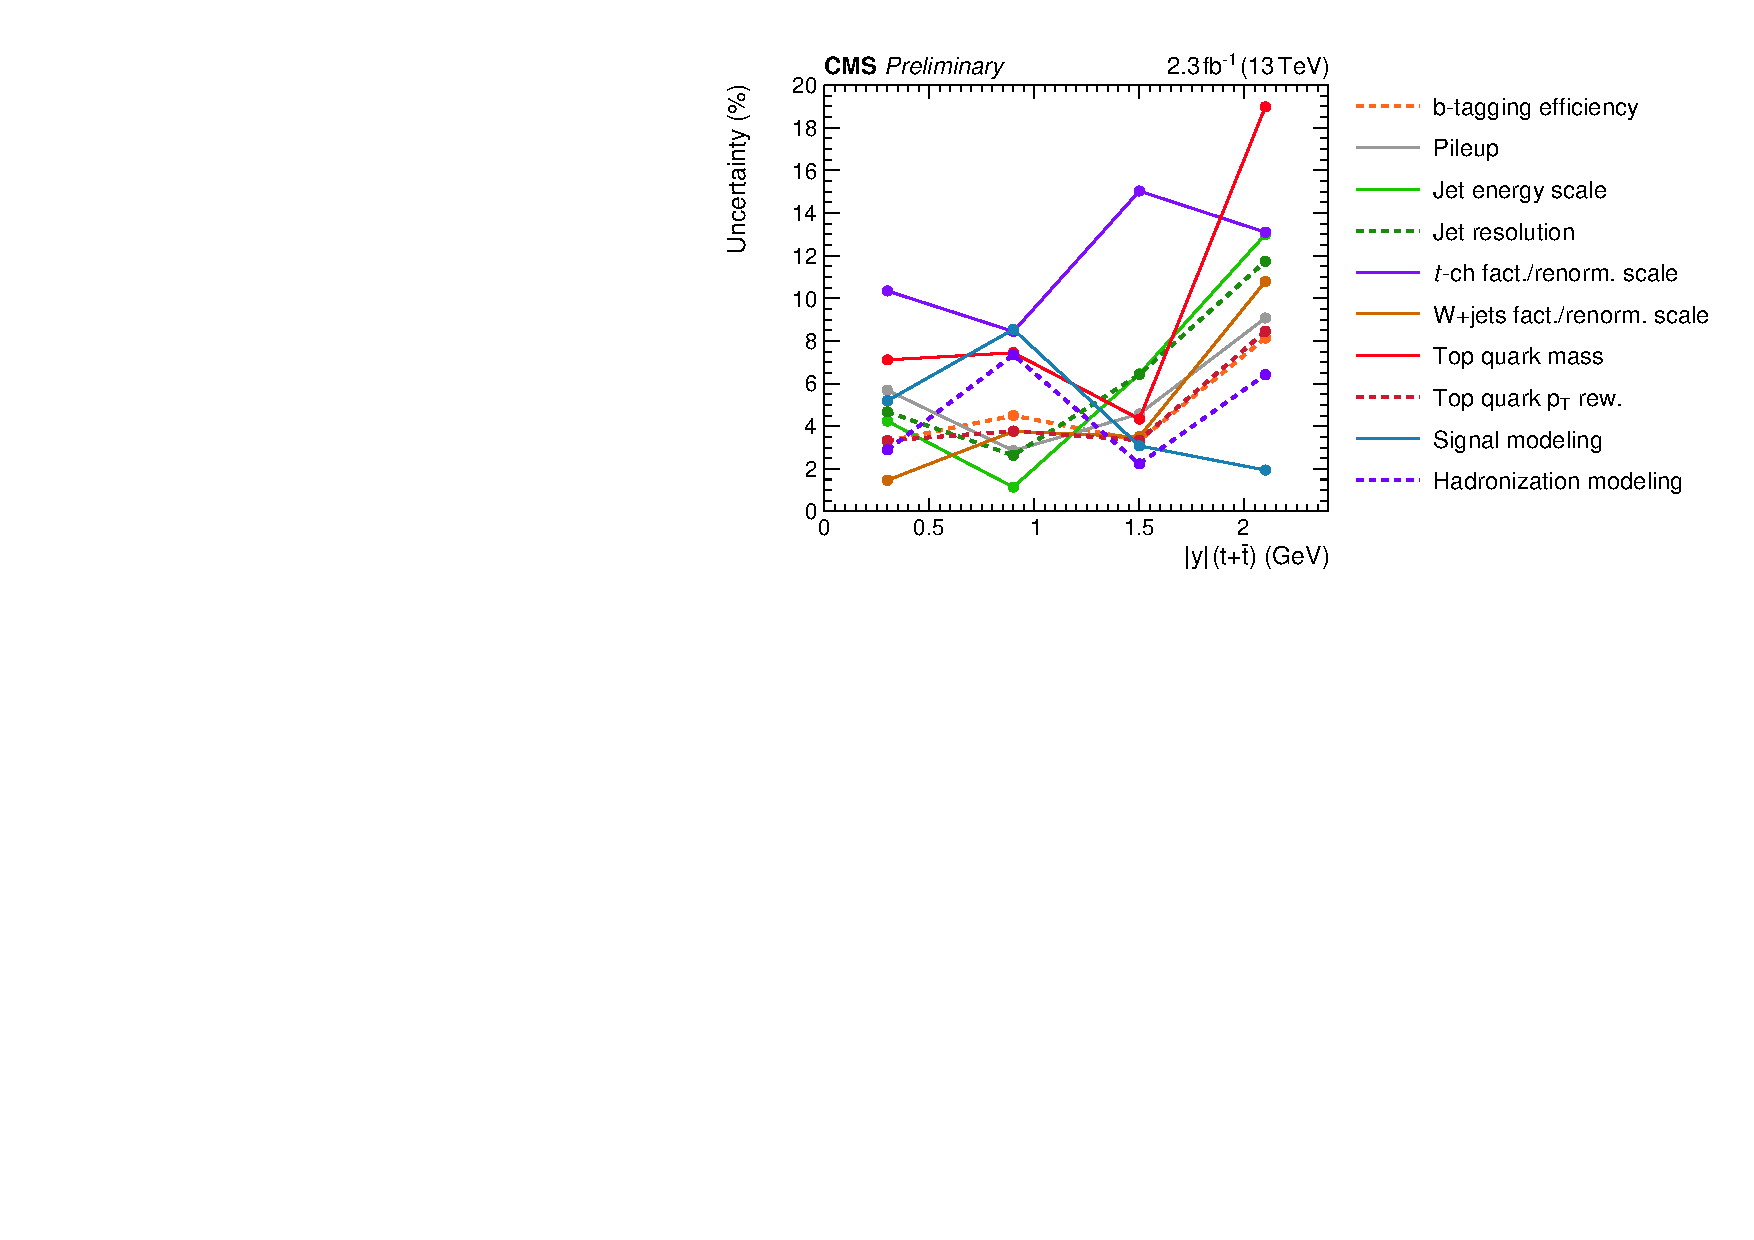
\includegraphics[width=0.9\textwidth]{figures/differential/unfolding/unfolded_top_y_unc.pdf}}
}

%##############################################
\section{Results}
%##############################################

\myfigure{\label{fig:diff13-top-unfolded} The figures are taken from Ref.~\cite{CMS-PAS-TOP-16-004}.}{
\subfloat[]{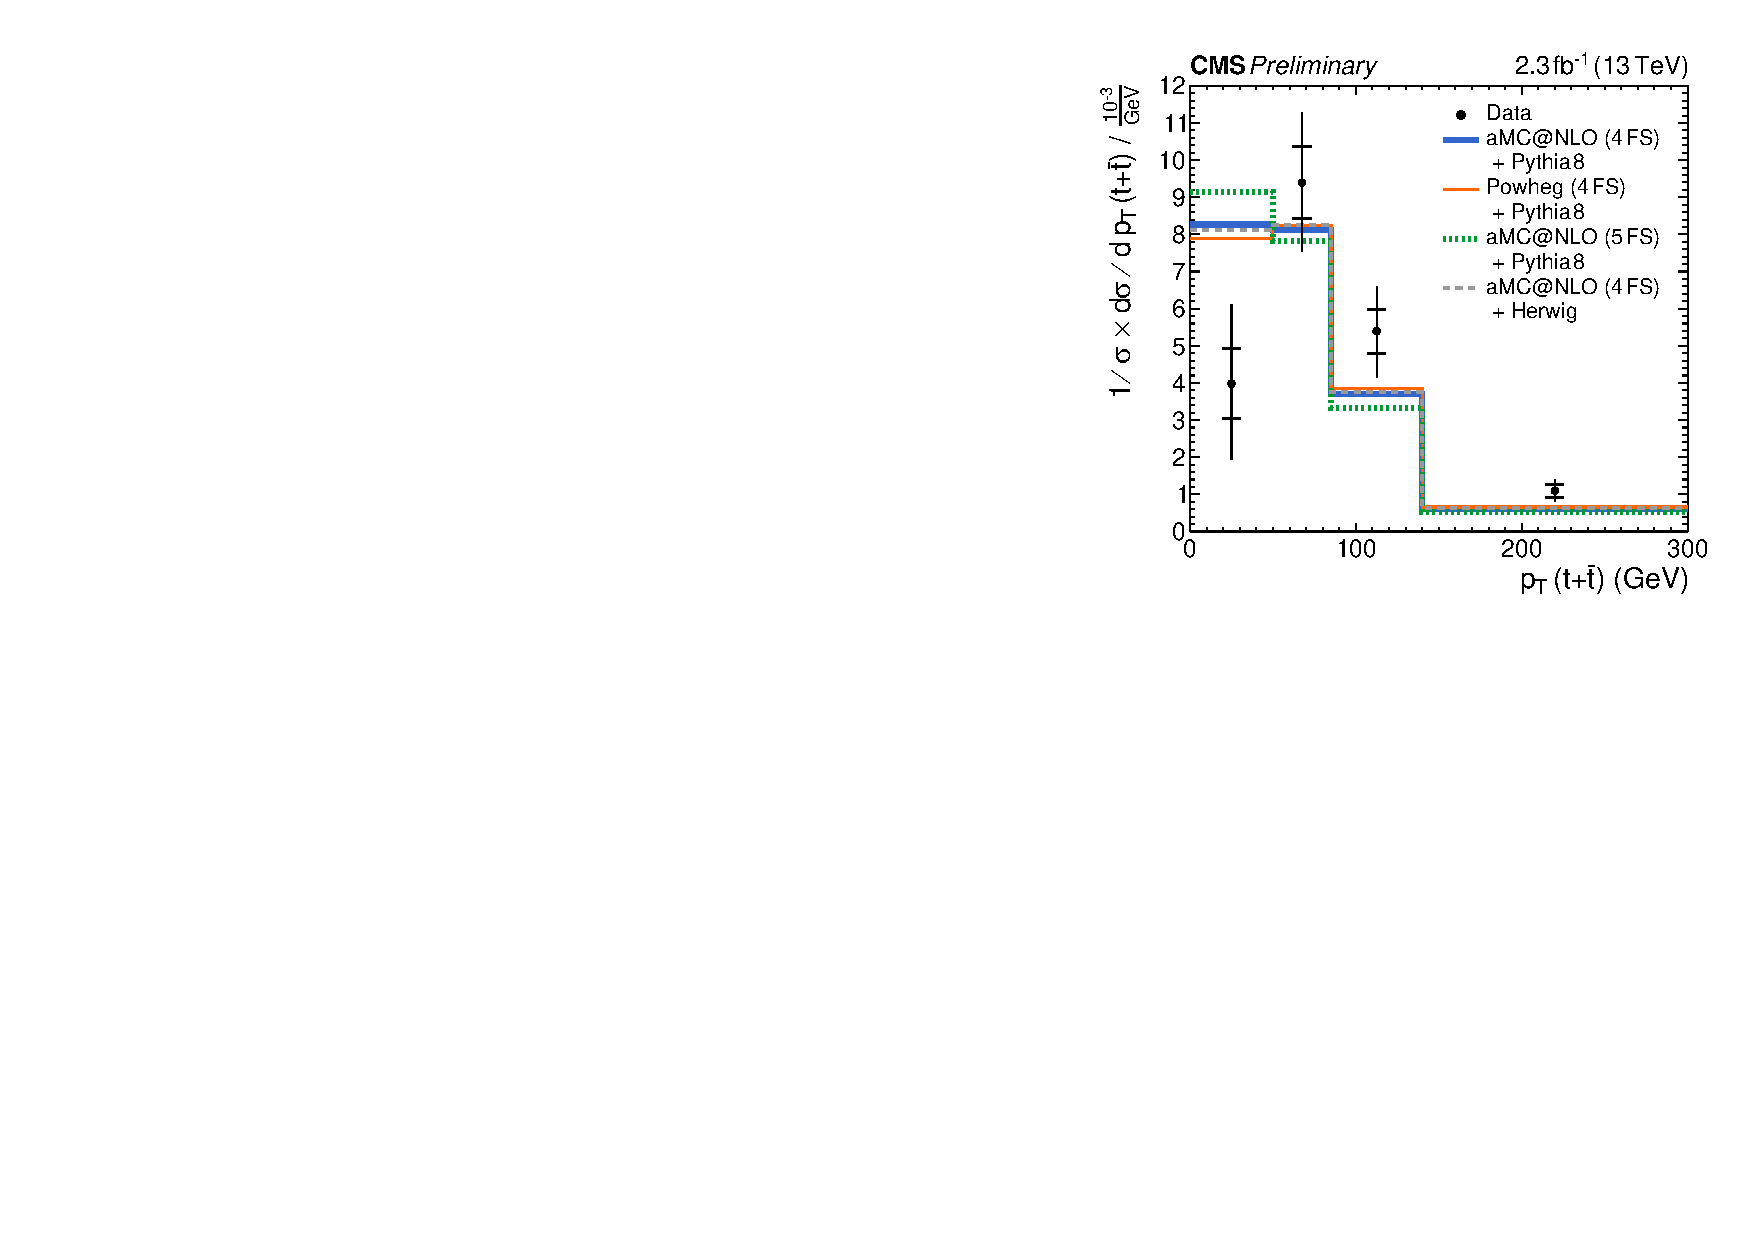
\includegraphics[width=0.48\textwidth]{figures/differential/pas/unfolded_top_pt.pdf}}
\hspace{0.02\textwidth}
\subfloat[]{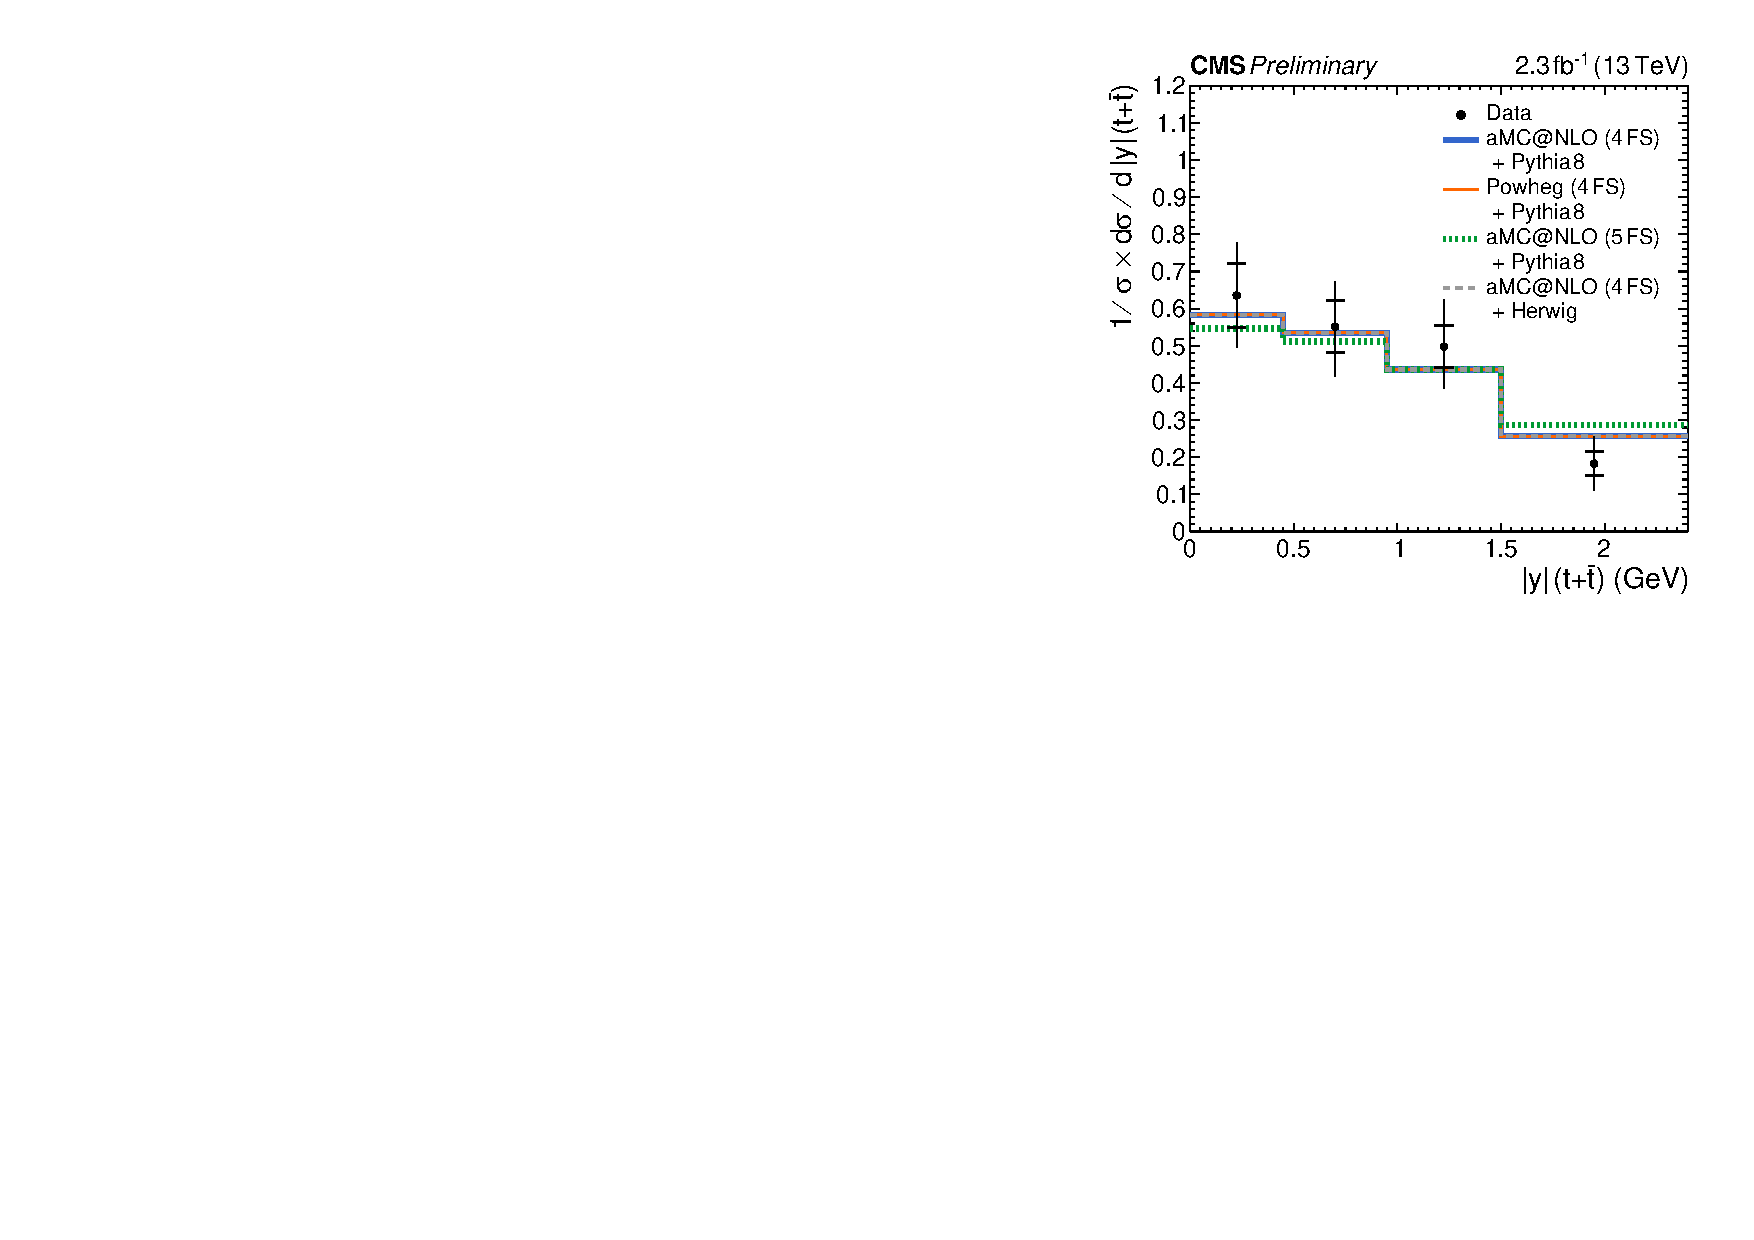
\includegraphics[width=0.48\textwidth]{figures/differential/pas/unfolded_top_y.pdf}}
}

\myfigure{\label{fig:diff13-top-unfolded-xcheck}Cross check of the top quark \pt differential cross section result by fitting the pseudorapidity distribution of the spectator jet instead of the \gls{bdt} discriminant.}{
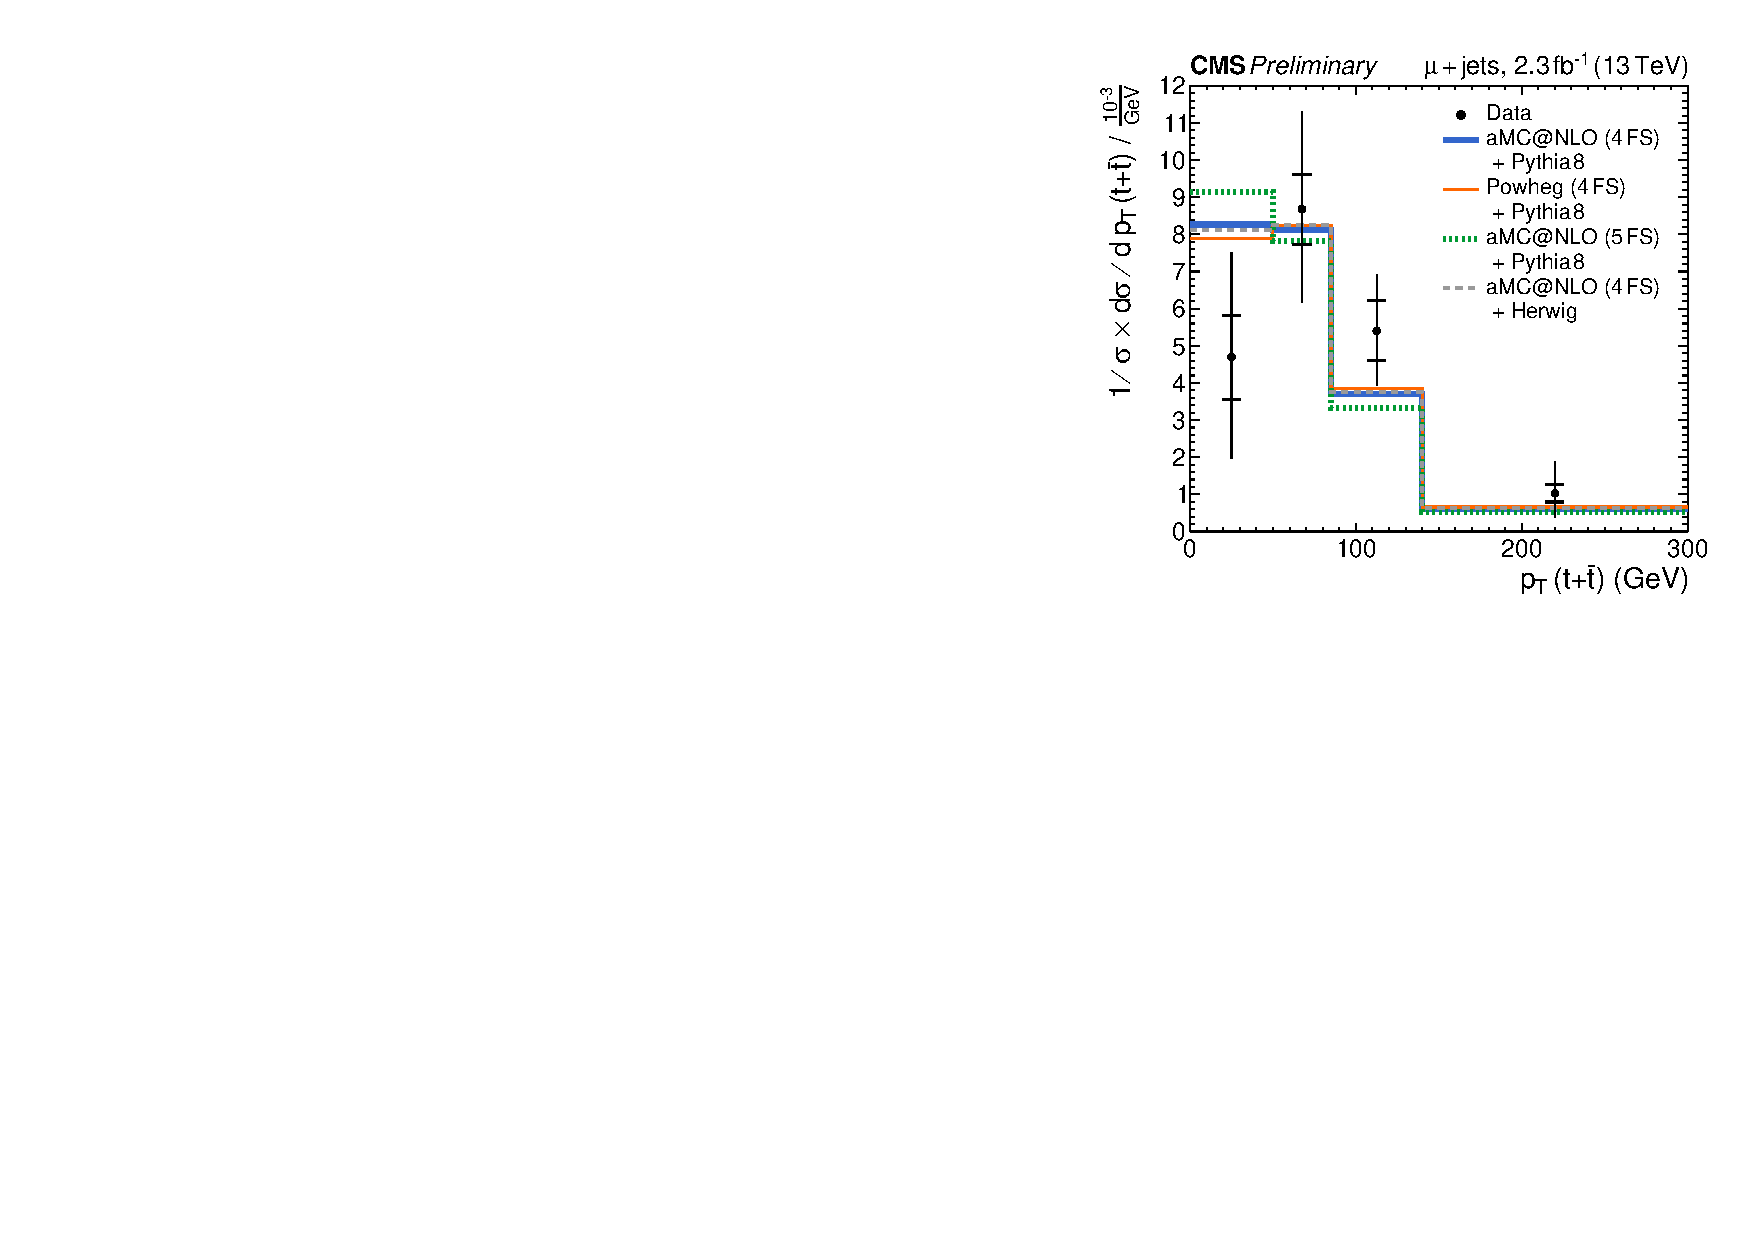
\includegraphics[width=0.48\textwidth]{figures/differential/pas/unfolded_top_pt_jeta.pdf}
}

